\documentclass[11pt,a4paper]{article}
\usepackage[utf8]{inputenc}
\usepackage[T1]{fontenc}
\usepackage{lmodern}
\usepackage[margin=2.5cm]{geometry}
\usepackage{graphicx}
\usepackage{microtype}
\usepackage{csquotes}
\usepackage[hidelinks]{hyperref}
\setlength{\parskip}{0.5em}
\setlength{\parindent}{0pt}

%% Generated from paper.md by scripts/paper_md_to_tex.py - do not edit by hand.
%% Edit paper.md and regenerate, so the two versions cannot diverge.

\title{Falsification-First Alpha Discovery: How Data Construction, Survivorship, Semantic Errors and Execution Constraints Create and Destroy Apparent Trading Opportunities}
\date{2026-10-11}
\author{}
\begin{document}
\maketitle


\textbf{Working paper, V2.} 2026-10-11. Revised after referee report V1.


\begin{quote}
\textbf{Relationship to V1.} V1 is frozen at commit \texttt{52a980a} (\texttt{paper.md} SHA-256 \texttt{1853bce0\ldots{}}) and is not edited. This is a separate document. Every material change from V1 is listed in \texttt{PAPER\_V2\_FREEZE.md} and traced to the referee concern that produced it. V2 claims \textbf{less} than V1, not more.
\end{quote}



\section*{Abstract}


Research on systematic trading strategies is normally defended against overfitting: out-of-sample testing, corrections for multiple testing, and pre-specification of the model. A substantial literature already establishes that these defenses are necessary and frequently insufficient --- that reported Sharpe ratios must be deflated by the number of trials [Bailey \& López de Prado 2014], that most published anomalies do not survive replication [Hou, Xue \& Zhang 2020], that analyst discretion alone generates dispersion comparable to sampling error [Menkveld et al. 2024], that missing delisting returns can carry an entire size effect [Shumway 1997; Shumway \& Warther 1999], and that leakage is the leading cause of irreproducibility in machine-learning-based science [Kapoor \& Narayanan 2023]. \textbf{What that literature documents less often is the cost, in sample size and in feasibility, of actually enforcing these requirements on a specific research program --- and what happens when enforcement makes a study impossible before it begins.}


We report that cost. Seventeen hypothesis families (H13--H19.2) drawn from a thirty-one-entry research registry were run on free public data under a protocol that gated data construction, semantics, point-in-time validity, identification and execution before any economic quantity was computed. We contribute four specific, auditable procedures and their measured outcomes. \textbf{(1) Venue-side archive asymmetry:} an exchange's own archive retains instruments its delisting removed, at a 0.0 pp retrieval differential between active and delisted pairs, which makes a survivorship-safer risk set \emph{constructible} from venue-owned history rather than only \emph{correctable} after the fact. \textbf{(2) A validated lifecycle universe with a measured recall denominator:} 201 full-asset delisting events, recall 0.9801 against candle-measured cessation, with all 60 unexplained non-announcements individually classified --- the validation method, not the event count, is the contribution. \textbf{(3) A pre-freeze full-pool common-support ceiling:} the complete eligible control pool was evaluated before the design was frozen and before any outcome column was opened, giving a median of 7 eligible matched controls per event date against a pre-registered floor of 20, with only 3 of 25 dates reaching the floor. \textbf{(4) Structural outcome blinding:} the data loader physically excluded price columns, so no outcome could have been inspected even accidentally, and this is auditable from source.


Two empirical cases bound what the procedures cost. A pre-registered predictive test positive in all eight rolling-origin folds (pooled $\Delta$PR-AUC +0.0270, +13.46\% relative) failed its frozen support criteria when the cluster-bootstrap interval [$-$0.0074, +0.0628] crossed zero and the single-use holdout reversed sign ($-$0.00753); we label this \texttt{PRE-REGISTERED NULL}, meaning \textbf{the pre-registered support criteria were not met}, and we state explicitly that an interval of this width does not demonstrate absence of effect. And 201 documented delisting events reduce to 32 that pass a coarse volume-based liquidity screen --- a screen, not an execution analysis, since no order book, spread, impact, fee, funding or latency measurement was available.


We report the full registry denominator, including the twelve families not analysed in detail and the eleven entries in which an economic quantity \emph{was} computed and the verdict came from it. We state which governance rules were in force at the start and which were added after a named failure; the program became progressively more falsification-first as failures accumulated, and we document that trajectory rather than asserting the mature protocol as a starting condition. We classify every decision threshold as theoretical, conventional or engineering judgement, and note that threshold sensitivity remains unmeasured.


\textbf{Keywords:} survivorship bias, point-in-time data, common support, pre-registration, execution feasibility, research methodology, cryptocurrency delisting.



\section*{1. Introduction}


\subsection*{1.1 What is already known}


The failure of systematic strategy research to replicate is not a new observation, and this paper does not claim it as one.


Four strands establish the background. First, model-selection inflation: a reported Sharpe ratio cannot be interpreted without the number of strategy variants tried, and Bailey and López de Prado's deflated Sharpe ratio makes that count an explicit input. Second, replication: Hou, Xue and Zhang compile 447 anomaly variables and report 286 (64\%) insignificant at the 5\% level once microcaps are handled by NYSE breakpoints and value weighting. Third, analyst discretion: Menkveld et al. give many independent teams the same data and the same hypothesis and measure the dispersion of their results --- variation that conventional standard errors do not capture. Fourth, data construction itself: Shumway documents that correct delisting returns are missing for most stocks delisted for negative reasons, and Shumway and Warther estimate a $-$55\% correction for performance-related Nasdaq delistings, after which the Nasdaq size effect does not survive.


Outside finance, Kapoor and Narayanan survey seventeen fields and 294 affected papers, find leakage to be the leading cause of irreproducibility in machine-learning-based science, and propose an eight-type leakage taxonomy. In causal inference, Petersen et al. establish that positivity violations --- subgroups that rarely or never receive the treatment of interest --- bias estimates, and distinguish violations that are structural from those that are artefacts of a finite sample.


Taken together, this literature already owns the claims that survivorship distorts returns, that leakage is pervasive and classifiable, that researcher discretion matters, that anomalies replicate poorly, and that common support must hold for a comparison to mean anything. \textbf{A paper that restated those claims would contribute nothing.}


\subsection*{1.2 The gap this paper addresses}


What the literature documents less often is the \textbf{cost of enforcement}: what it takes, in a specific research program, to satisfy these requirements before an economic result is computed, and what remains testable afterwards.


That question has an unusual property. It can only be answered by a program willing to report what enforcement destroyed, including the studies that enforcement made impossible --- which is exactly the material that publication selects against. The positivity literature diagnoses violations on the analysed sample, after the study exists. The leakage literature audits published work, after the claims exist. The replication literature re-estimates published anomalies, after publication. None of them reports the research that never reached a result because a requirement was enforced in advance.


This paper reports that. The contribution is four auditable procedures and what they measured.


\subsection*{1.3 Contributions}


\textbf{Four procedures, and the measurements they produced.}


\begin{enumerate}
\item \textbf{Venue-side archive asymmetry (\S{}5.1).} The survivorship literature documents the bias inside
\end{enumerate}
   vendor databases and supplies corrections. We measure the other side: the venue that delisted the    instrument retains its history, at a \textbf{0.0 pp} retrieval differential between active and delisted    spot pairs, with 1,936 delisted symbols retaining candles. The claim is bounded: this makes a    survivorship-safer risk set \emph{constructible} from venue-owned history without paid data. It is not    a discovery of survivorship bias, and it is a property of one venue measured against two others.

\begin{enumerate}
\item \textbf{A validated lifecycle universe with a measured recall denominator (\S{}5.3).} 201 full-asset
\end{enumerate}
   delisting events over nine years, with recall \textbf{0.9801} against an independent, candle-measured    definition of cessation, and all 60 assets that stopped being served without an announcement    individually classified. The transferable part is the validation method --- measuring recall against    a denominator derived from market data rather than from the document source being validated.

\begin{enumerate}
\item \textbf{A pre-freeze full-pool common-support ceiling (\S{}8.2).} Before freezing a matched design and
\end{enumerate}
   before opening any outcome column, the complete eligible control pool was evaluated at every    candidate event date. The median number of eligible matched controls was \textbf{7} against a    pre-registered floor of 20, and only \textbf{3 of 25} dates reached the floor. The procedural claim is    that common-support feasibility can be bounded on the full eligible population \emph{before} an outcome    is opened. Positivity theory is not claimed as novel; the pre-freeze, full-pool, outcome-blind    application is the contribution.

\begin{enumerate}
\item \textbf{Structural outcome blinding (\S{}8.3).} The feasibility loader requested four non-price columns;
\end{enumerate}
   the OHLC columns never entered memory. No return, VWAP, abnormal score, basis or funding direction    could have been computed even by accident, and this is checkable from the source rather than    asserted. Blinding is not novel; blinding that is auditable from data-access code is the claim.


\textbf{Two bounded empirical results} (\S{}6, \S{}7) show what the procedures cost in sample size, and a full registry denominator (\S{}4) shows what fraction of the program they touched.


\subsection*{1.4 Two definitions used throughout}


\textbf{Point-in-time (PIT).} A quantity is point-in-time with respect to a decision at time t if it is constructible using only records whose publication or observation time precedes t. A value that is numerically correct and correctly dated may still fail this test, if the rule that produced it used information published after t (\S{}10).


\textbf{Common support.} Two groups have common support over a covariate set if, for every covariate stratum that occurs in the treated group, the comparison group also contains units. Where an exact matching rule is used, common support is a counting condition: the matched cell must be non-empty at the required size. This is the finite-sample form of the positivity assumption [Petersen et al. 2012].


\subsection*{1.5 What this paper does not claim}


It does not claim that the economic hypotheses examined are false; in most families they were never tested. In the detailed cases examined here, the decisive failure often occurred before or outside model selection; that is a statement about four retrospectively selected cases, not about systematic research in general. It does not claim that the model layer is unimportant --- \S{}4 reports eleven registry entries in which an economic quantity was computed and the verdict came from it. It does not claim that the governance protocol described in \S{}2 was in force from the start; \S{}2B documents when each rule was added and which failure produced it. And its detailed cases were selected retrospectively, which \S{}4.1 states explicitly.



\section*{2. Research governance, and when each rule appeared}


The referee's sharpest objection to V1 was that it presented a mature protocol as the frame for work that predated most of it. That objection was correct. This section is split accordingly.


\subsection*{2A. Rules in force at the start of the reported program}


These rules governed the earliest families in the registry and are visible in the first pre-registration documents and commits.


\begin{center}
\footnotesize
\begin{tabular}{p{0.460\linewidth}p{0.460\linewidth}}
\hline
\textbf{rule} & \textbf{evidence} \\
\hline
\textbf{Pre-registration before any P\&L.} The hypothesis, data, rule and decision criteria are written and committed before an aggregate return is computed. & \texttt{docs/alpha\_sprint/PREREGISTRATION.md}, first families dated 2026-09-18 \\
\textbf{Explicit, numeric decision criteria} fixed in the pre-registration, with a stated hurdle. & same; cycle-2 hurdle stated in the ledger \\
\textbf{Train / validation / holdout separation} with the holdout reported separately. & early family gates report validation and holdout figures separately \\
\textbf{A written verdict vocabulary}: \texttt{REJECT}, \texttt{WATCH}, \texttt{RESEARCH}, \texttt{PROCEED}. & hypothesis ledger, cycle 1 \\
\textbf{Red team before pre-registration} --- an adversarial document attacking the hypothesis before it is registered. & \texttt{H9\_RED\_TEAM.md}, \texttt{H10}--\texttt{H13} red-team documents \\
\textbf{Append-only experiment ledger} with one row per family and a dated verdict. & \texttt{docs/alpha\_sprint/HYPOTHESIS\_LEDGER.md} \\
\textbf{Costs and executable prices before P\&L} (prediction-market families use executable asks, not mid). & H9 gate: edge measured at executable asks \\
\hline
\end{tabular}
\end{center}


\subsection*{2B. Rules added after a specific failure}


Each row names the family where the rule first appears, the failure that produced it, and the commit.


\begin{center}
\footnotesize
\begin{tabular}{p{0.184\linewidth}p{0.184\linewidth}p{0.184\linewidth}p{0.184\linewidth}p{0.184\linewidth}}
\hline
\textbf{rule} & \textbf{first introduced} & \textbf{triggering failure} & \textbf{commit (date)} & \textbf{methodological lesson} \\
\hline
\textbf{Data gate before any P\&L}, with named criteria and a pass count & H14 family (2026-09-27) & a universe was assembled whose fields could not be validated to a usable accuracy & \texttt{61f0bc8}, \texttt{7c44e67} & extraction accuracy is a gate, not a nuisance \\
\textbf{Two-pass gold sets, PASS 1 persisted before PASS 2 begins}, with reviewer churn reported & H14.1 / H15 & field accuracy claims had no independent denominator & \texttt{7c44e67} (2026-09-27), \texttt{cb722dd} (2026-09-28) & a self-scored extraction is not validation \\
\textbf{Outcome-differential missingness audit at every join} & H17.0 & identity passed at 98--99\% while price coverage failed, and the coverage correlated with the outcome & \texttt{e96ba10} (2026-09-28) & survivorship removed upstream reappears downstream \\
\textbf{Label-free survivorship split} (partition by an outcome-independent proxy) & H17.0 & the fate labels themselves were found unreliable for one class & \texttt{e96ba10} & do not audit a label with the label \\
\textbf{Source coverage measured against the source's own reported total}, with a guard that refuses to write a universe below a stated fraction & H18.1b & a transient empty page truncated a catalog harvest and silently deleted four years of events & \texttt{27c3283} (2026-10-10) & a clean horizon at a round date is a coverage artefact until proven otherwise \\
\textbf{Asset-era keying} --- identity is (asset, era), never ticker alone & H18.1b & a ticker-keyed join substituted a different asset that had taken the ticker later & \texttt{27c3283} & a ticker is a lease, not an identity \\
\textbf{Served candle ≠ traded market} --- materiality requires trades, not candles & H18.1b & post-cessation candles were served for pairs that had stopped trading & \texttt{27c3283} & data availability is not market activity \\
\textbf{SHA-256 pre-registration freeze}, hashed and committed before execution & H18.3 & the program had pre-registrations but no cryptographic evidence they predated results & \texttt{522bafb} (2026-10-10) & a commit proves order; a hash proves content \\
\textbf{Classification-level leakage audit} --- re-derive every categorical label under a strictly backward window & H18.3 amendment 01 & 28.7\% of removal classes had been assigned using post-decision information while every value and date was correct & \texttt{203390b} (2026-10-10) & auditing values and dates does not audit classification \\
\textbf{Administrative censoring and event-sharing embargo} measured on landmark dates & H18.3 & the originally specified split boundaries shared 41 of 86 holdout outcome events & \texttt{522bafb} & date boundaries do not separate events when the outcome has a horizon \\
\textbf{Holdout directional veto} --- a positive support label requires a positive holdout delta & H18.3 amendment 01 & the amendment anticipated that development and holdout could disagree in sign & \texttt{203390b} & decide in advance what a sign reversal means \\
\textbf{Point-in-time instrument existence} --- current instrument lists may not be used as history & H19.0 & a live API list would have asserted instruments that did not exist at the event & \texttt{320ce41} (2026-10-10) & the present is not a sample of the past \\
\textbf{Identity guard that rejects a mapping with no asset-era at T0} & H19.0 & a ticker-keyed mapping pointed at an asset that acquired the ticker four years after the event & \texttt{320ce41} & enforce the keying rule in code, not in prose \\
\textbf{Structural no-price feasibility checks} --- pre-freeze work loads only non-price columns & H19.1, H19.2 & zero-return claims were declarative and unverifiable & \texttt{564baf8}, \texttt{42f35df} (2026-10-10) & make the guarantee a property of the code \\
\hline
\end{tabular}
\end{center}


\textbf{The correct headline is that the program became progressively more falsification-first as failures accumulated.} Most of \S{}2B's rules are the output of H14--H19, not their input. The earliest families in the registry ran under \S{}2A alone, without hashed pre-registrations, without gold-set discipline, and without the leakage and identity audits. Any reading in which the full protocol governed the whole program is wrong, and the trajectory is itself part of the evidence: a research program's protocol is revised by its own failures, and the revisions are dated.


\subsection*{2C. Outputs that are not failures}


Two terminal states are treated as valid results rather than as absence of a result.


\texttt{NO\_TEST} means a gate specified in advance was not met and no economic test was run. It makes no claim about the economic hypothesis. \texttt{NO\_TRADE} means the rule produced no position, or no tradable instrument existed --- which is not a zero return but an absence of a position. Collapsing either into "the strategy did not work" destroys the distinction that \S{}3 depends on.



\section*{3. A taxonomy of research outcomes}


\begin{center}
\footnotesize
\begin{tabular}{p{0.307\linewidth}p{0.307\linewidth}p{0.307\linewidth}}
\hline
\textbf{label} & \textbf{meaning} & \textbf{what may be concluded} \\
\hline
\texttt{PROMOTED} & passed every pre-registered criterion and moved to paper trading & the rule survived this program's tests \\
\texttt{IMPLEMENTATION REJECT / ECONOMIC QUESTION UNRESOLVED} & tested against pre-registered bars and rejected, where the test could not settle the economics & the implementation does not meet the bar; the economic question may remain open \\
\texttt{ECONOMIC REJECT} & tested and rejected, with the economic quantity computed & the hypothesis as specified does not pay under the stated bar \\
\texttt{PRE-REGISTERED NULL} & the design and data survived; the pre-registered support criteria were not met & the claim is not supported \textbf{at this sample size}; absence of effect is not demonstrated \\
\texttt{DATA-GATE FAIL / UNTESTED} & a data or semantic gate failed; no economic test ran & nothing about the economics \\
\texttt{INFRASTRUCTURE BLOCKED} & the substrate was unavailable at the required quality & nothing about the economics \\
\texttt{IDENTIFICATION BLOCKED} & data adequate; the design does not identify the effect & nothing about the economics \\
\texttt{EXECUTION / CAPACITY FAIL} & the event is real and the instrument traded; capacity or liquidity screening fails & the opportunity is not accessible at the stated size; \textbf{not} a profitability result \\
\texttt{OPEN} & universe built, no hypothesis selected & nothing \\
\texttt{WATCH / RESEARCH} & inconclusive, carried forward & nothing yet \\
\hline
\end{tabular}
\end{center}


Only the first four rows carry information about an economic claim.



\section*{4. The full registry denominator}


\subsection*{4.1 Case selection was retrospective}


\begin{quote}
\textbf{The four detailed case studies were selected retrospectively for methodological informativeness. Hypothesis selection within families and case selection for this manuscript are different processes.}
\end{quote}


Hypothesis selection inside each family was pre-registered, and from H18.3 onward it is auditable by hash and commit order. Case selection for this manuscript was not: the thesis was formed after the families ran, and the four cases were chosen because they illustrate it. Had the families produced different outcomes, the protocol would be the same --- it is recorded in dated, committed documents --- but this paper would not be, because its cases were chosen for what they show.


The remainder of this section reports the denominator that makes that selection visible.


\subsection*{4.2 All families, H1 to H19.2}


Thirty-one registry entries across ten research cycles. "Economic outcome computed" means an aggregate return, edge or P\&L figure was produced. Sources: \texttt{docs/alpha\_sprint/HYPOTHESIS\_LEDGER.md}, the per-family gate artefacts, and the git history.


\begin{center}
\footnotesize
\begin{tabular}{p{0.092\linewidth}p{0.092\linewidth}p{0.092\linewidth}p{0.092\linewidth}p{0.092\linewidth}p{0.092\linewidth}p{0.092\linewidth}p{0.092\linewidth}p{0.092\linewidth}p{0.092\linewidth}}
\hline
\textbf{\#} & \textbf{family} & \textbf{question} & \textbf{stage reached} & \textbf{terminal state} & \textbf{failure class} & \textbf{econ. outcome computed} & \textbf{pre-registered} & \textbf{holdout used} & \textbf{reference} \\
\hline
H1 & perp/quarterly regime switching & does a regime switch between perpetual and quarterly carry pay? & full test & \texttt{REJECT} & economic & \textbf{yes} & yes & yes & \texttt{PREREGISTRATION.md}, 2026-09-18 \\
H2 & funding settlement timing & is there an edge around funding settlement? & partial test & \texttt{WATCH} after H2.1--2.3 & inconclusive & \textbf{yes} & yes & --- & \texttt{94052bf} \\
H3 & liquidation reversal (audit) & do liquidation cascades revert? & audit & \texttt{WATCH} $\rightarrow$ H3.1 & inconclusive & no & yes & --- & \texttt{PREREGISTRATION.md} \\
H3.1 & cascade exhaustion vs continuation & does cascade exhaustion predict reversal? & full test & \texttt{REJECT} & economic & \textbf{yes} & yes & yes & \texttt{18c3f65} \\
H4 & cross-sectional funding/basis/momentum & does a cross-sectional carry/momentum book pay? & full test & \texttt{REJECT} / \texttt{WATCH} & economic & \textbf{yes} & yes & yes & \texttt{PREREGISTRATION.md} \\
H5.1 & CEX↔DEX funding fragmentation & is fragmented funding arbitrageable? & full test & \texttt{REJECT} & economic & \textbf{yes} & yes & yes & \texttt{fb9e6d1} \\
H6.1 & options volatility risk premium & is the VRP harvestable at retail cost? & full test & \texttt{REJECT} & economic & \textbf{yes} & yes & yes & \texttt{16cc502} \\
H7.1 & prediction-market logical arbitrage & do logically linked contracts admit arbitrage? & full test & \texttt{REJECT} & economic & \textbf{yes} & yes & yes & \texttt{a8639ae} \\
H8.1 & cross-asset medium-horizon trend & does slow multi-asset trend survive falsification? & full test & \textbf{\texttt{PROMOTED} $\rightarrow$ paper portfolio} & --- & \textbf{yes} & yes & yes & \texttt{e771727}, \texttt{0e865bd} \\
H8.2 & equal-risk / risk-off overlay falsifications & do alternative allocations beat the champion? & falsification of alternatives & \texttt{KEEP H8.1} & --- & \textbf{yes} & yes & --- & \texttt{032fc25} \\
H9 & prediction-market favourite premium & do favourites at executable asks pay? & full test & \texttt{REJECT} & economic (cost) & \textbf{yes} & yes & yes & \texttt{756719f}, \texttt{77a760a} \\
H10 & odd-lot priority in issuer tender offers & does odd-lot priority pay for small capital? & full test & \texttt{REJECT} & economic & \textbf{yes} & yes & yes & \texttt{5a7c7c1}, \texttt{7db3245} \\
H11 & post-spin forced selling & do index-fund orphans revert after forced flow? & full test & \texttt{REJECT} & economic & \textbf{yes} & yes & yes & \texttt{6e5903f}, \texttt{482a2e0} \\
H12 & public-company liquidation discount & does a conservative NAV discount pay? & data phase & \texttt{RESEARCH (data)} & data coverage & partial & yes & --- & \texttt{e2d5f71}, \texttt{5756040} \\
H13 & net-nets / cash shells & do filings separate cheap-ignored from cheap-dying? & full test & \textbf{\texttt{IMPLEMENTATION REJECT / ECONOMIC QUESTION UNRESOLVED}} & data construction & \textbf{yes} & yes & yes & \texttt{aca53bf}, \texttt{9e73558} \\
H14 & B3 deep special situations & which Brazilian corporate events are testable? & universe only & \textbf{\texttt{OPEN}} & --- & no & no & --- & \texttt{61f0bc8} \\
H14.1 & B3 takeover-offer terms & can offer terms be extracted reliably? & gate & \texttt{DATA-GATE FAIL} & semantics & no & no & --- & \texttt{7c44e67} \\
H14.2 & B3 judicial reorganisation & can reorganisation states be extracted? & gate (1 of 7) & \texttt{DATA-GATE FAIL} & semantics & no & no & --- & \texttt{58bd03f} \\
H14.3 & B3 recapitalisations and rights & can dilution events be reconstructed? & gate (0 of 9) & \texttt{DATA-GATE FAIL} & data construction & no & no & --- & \texttt{eabd336} \\
H15 & Schedule 13D activist & can activist intent and outcome be extracted? & gate (5 of 22) & \texttt{DATA-GATE FAIL / UNTESTED} & semantics & no & no & --- & \texttt{cb722dd} \\
H16.1 & FDA / PDUFA binary catalysts & can an ex ante decision universe be built? & gate (2 of 23) & \texttt{DATA-GATE FAIL / UNTESTED} & identity, dates, joins & no & no & --- & \texttt{dcefafe} \\
H17.0 & historical market data for Form 4 & does usable price history exist for the seed? & gate (14 of 32) & \texttt{INFRASTRUCTURE BLOCKED} & data construction & no & no & --- & \texttt{e96ba10} \\
H18.0 & three-venue delisted-OHLCV probe & does any venue serve delisted spot history? & gate (2 of 3 venues required) & \texttt{INFRASTRUCTURE BLOCKED} & substrate & no & no & --- & \texttt{6f7dbf4} \\
H18.0b & venue substrate confirmation & does this venue preserve delisted pairs? & gate (14 of 14) & \texttt{PASS} (substrate) & --- & no & no & --- & \texttt{55f68ec} \\
H18.1 & spot lifecycle semantic audit & is a removal notice an asset delisting? & gate (11 of 12) & \texttt{PARTIAL PASS} & semantics & no & no & --- & \texttt{2a746cc} \\
H18.1b & full-delisting universe expansion & was the event universe truncated? & gate (19 of 19) & \texttt{STRONG PASS} & --- & no & no & --- & \texttt{27c3283} \\
H18.2 & hypothesis selection & which delisting hypothesis is testable? & selection & \texttt{SELECT H18-P1} & --- & no & n/a & --- & \texttt{45d575d} \\
H18.3 & route contraction $\rightarrow$ 365-day delisting risk & does route history add incremental information? & \textbf{full pre-registered test} & \textbf{\texttt{PRE-REGISTERED NULL}} & --- & no (no return; PR-AUC only) & \textbf{yes, hashed} & \textbf{yes, opened once} & \texttt{522bafb}, \texttt{203390b}, \texttt{4aa4180} \\
H19.0 & execution / shortability gate & did a tradable short exist at the announcement? & gate (12 of 15) & \textbf{\texttt{PARTIAL PASS} / capacity fail} & execution & no & no & --- & \texttt{320ce41} \\
H19.1 & derivative price-discovery selection & is a derivative-lead hypothesis testable? & selection & \texttt{SELECT H19-P3A} + 3 modifications & --- & no & n/a & --- & \texttt{564baf8} \\
H19.2 & derivative-specific pre-delisting discovery & does the derivative lead spot before the announcement? & pre-freeze feasibility & \textbf{\texttt{BLOCKED BEFORE FREEZE / IDENTIFICATION FAIL}} & identification & no (no price read) & \textbf{no --- never frozen} & no & \texttt{42f35df} \\
\hline
\end{tabular}
\end{center}


\subsection*{4.3 Terminal-state distribution}


\begin{center}
\footnotesize
\begin{tabular}{p{0.307\linewidth}p{0.307\linewidth}p{0.307\linewidth}}
\hline
\textbf{terminal state} & \textbf{count} & \textbf{families} \\
\hline
\texttt{PROMOTED} & \textbf{1} & H8.1 \\
\texttt{ECONOMIC REJECT} (economic quantity computed) & \textbf{9} & H1, H3.1, H4, H5.1, H6.1, H7.1, H9, H10, H11 \\
\texttt{IMPLEMENTATION REJECT / ECONOMIC QUESTION UNRESOLVED} & \textbf{1} & H13 \\
\texttt{PRE-REGISTERED NULL} & \textbf{1} & H18.3 \\
\texttt{DATA-GATE FAIL / UNTESTED} & \textbf{5} & H14.1, H14.2, H14.3, H15, H16.1 \\
\texttt{INFRASTRUCTURE BLOCKED} & \textbf{2} & H17.0, H18.0 \\
\texttt{IDENTIFICATION BLOCKED} & \textbf{1} & H19.2 \\
\texttt{EXECUTION / CAPACITY FAIL} & \textbf{1} & H19.0 \\
\texttt{OPEN} & \textbf{1} & H14 \\
\texttt{WATCH / RESEARCH} (inconclusive, carried) & \textbf{3} & H2, H3, H12 \\
construction or substrate \texttt{PASS} (not hypotheses) & \textbf{3} & H18.0b, H18.1, H18.1b \\
hypothesis selection (not a verdict) & \textbf{2} & H18.2, H19.1 \\
falsification of alternatives & \textbf{1} & H8.2 \\
\textbf{total registry entries} & \textbf{31} &  \\
\hline
\end{tabular}
\end{center}


\subsection*{4.4 What the denominator does to the paper's thesis}


Three facts in this table cut against the story the detailed cases tell, and we report them rather than omit them.


\textbf{First, an economic quantity was computed in eleven entries, and in nine of them the verdict came from that computation.} H1, H3.1, H4, H5.1, H6.1, H7.1, H9, H10 and H11 were tested to completion and rejected on their economics or their costs, not on a data gate. H9 is explicit: favourites at 95--99 cents with at least seven days remaining resolve YES 91\% of the time, and the net edge at executable asks is $-$5.8 cents in validation and $-$5.7 cents on the holdout. That is a cost-and-pricing rejection reached by running the test, and no amount of data-construction discipline would have produced it in advance. \textbf{Any claim that pre-model failure is the typical case is not supported by this registry.} What the registry supports is narrower: pre-model failure was decisive in the families that reached the later cycles, and those are the families this paper examines in detail.


\textbf{Second, the single promoted family did not clear the return hurdle it was later held to.} H8.1 passed all eight pre-registered criteria and moved to a paper portfolio; the ledger records that it was archived on 2026-09-20 as a defensive / risk-overlay candidate because its 6--7\% annual return fell below a 12.7\% hurdle applied in a later sponsor reset, and that the paper portfolio continues unchanged. The framework's one promotion is therefore a conditional one. We state this rather than cite H8 as evidence that the process promotes hypotheses.


\textbf{Third, the cycles are not independent attempts at the same question.} Cycles 1--4 are strategy families with completed tests; cycles 5--10 are increasingly dominated by whether the data could support a test at all. That shift is partly a property of the domains chosen --- regulatory filings and venue archives rather than liquid futures --- and partly a property of the protocol tightening, which \S{}2B dates. Both readings are available and the data here cannot separate them.



\section*{5. Data construction before modelling}


\subsection*{5.1 Venue-side archive asymmetry}


The survivorship literature documents the problem from the consumer's side: Shumway shows that CRSP omits delisting returns for most negative delistings, and Shumway and Warther estimate the correction and show the Nasdaq size effect does not survive it. In cryptocurrency, Ammann et al. document a 39.5\% attrition rate over 2014--2021 and attribute the bias explicitly to reliance on aggregators that provide historical data only for currently listed assets.


We measure the other side. A three-venue probe required two of three venues to pass a nine-criterion substrate gate; the probe \textbf{failed} (4 of 9, 1 of 9 and 2 of 9), and that failure is the reported verdict. Inside it is the measurement that matters: one venue's active-versus-delisted retrieval differential is \textbf{0.0 pp} --- 28 of 30 active pairs and 28 of 30 delisted pairs retrieved, delisted hourly completeness 100\%, and no candles served after the delisting instant. A deeper confirmation run passed \textbf{14 of 14} criteria and established 1,403 unique pairs with both a symbol and a stated trading end; the lifecycle audit later resolved 2,965 symbols of which \textbf{1,936 delisted symbols retain history}.


\textbf{The bounded claim.} A venue that publishes its own archive retains what an aggregator has no commercial reason to keep, which makes a survivorship-safer risk set \emph{constructible} from venue-owned history, without paid data. This is not a discovery of survivorship bias; it is a measurement of where the record survives. It is also one venue measured against two that did not pass, so it is a statement about this venue's archive policy, not about exchanges in general.


\subsection*{5.2 Pair removal is not asset delisting}


Of \textbf{1,422 pair-removal events}, resolving into \textbf{1,271 asset-lifecycle episodes} across 532 assets, only \textbf{102 pair events and 84 episodes} are an asset leaving spot entirely --- \textbf{7.2\%}. The remainder are minor pair removals (688), quote migrations (510), fiat pair removals (95) and partial delistings (25). Treating "delisting notice" as one event type would have produced a sample in which 93\% of events are not the event the research intended to study.


The gate passed 11 of 12 criteria, failing only on category viability: at 84 episodes the full-delisting category fell below its pre-specified minimum of 100. The audit also recorded that the documentary period begins 2022-02-17 and that earlier years are \textbf{unavailable, never zero events}.


\subsection*{5.3 The catalog is not the population}


The validated universe is \textbf{201 asset-level full-delisting events} across nine calendar years (2018-10-12 to 2026-09-24), against the 84 the previous construction held --- \textbf{119 missed}. The decomposition: 75 in a different catalog category, 39 predating the catalog used, 5 visible only in the pair universe. Eighty-two of the 84 earlier episodes appear in the new universe; the two that do not (AUD, GBP) are fiat quote assets.


\textbf{The contribution is the validation, not the count.} An expanded event count proves nothing by itself --- a looser classifier also expands it. What makes the universe usable is a denominator constructed independently of the document source: recall \textbf{0.9801} measured against assets whose candles \emph{stopped being served}, which is a market-data fact rather than an announcement fact. Of 257 assets that stopped being served, 197 carry a full-delisting announcement and the remaining 60 are individually classified --- 34 pair removals only, 11 official rebrands or merges, 7 quote assets, 4 with no official record found, and 4 ticker reuses --- leaving \textbf{4 true false negatives}. Route validation independently confirms zero remaining routes for 189 events. A gold set of 100 events with 40 double-reviewed returned all-field accuracy of 1.0 and reviewer churn of 0.0; the audit itself records that several PASS-1 fields are partly self-confirming and that the independent evidence is the PASS-2 re-fetch and the rebuilt route state.


Two diagnostics sit below their 0.99 bar, at \textbf{0.9851} and \textbf{0.9847}, and are named rather than smoothed. Both are the same three events --- OST, RCN and WPR, all with a stated cessation of 2021-07-16 --- where the venue continued trading materially for three days past the instant its own notices state. The recorded dates are faithful to the documents; the venue's behaviour was not.


Reaching this universe required repairing defects described in \S{}10 and Table 3. \textbf{Finding one's own defect carries no information about markets}, and none of those repairs is presented as a result.


\subsection*{5.4 Survivorship migrates downstream}


A separate family built its seed from filings rather than from a current security list: 851,552 insider transaction records across 17 quarters produce 1,870 issuer-date observations over 1,579 issuers. The identity layer passes --- point-in-time symbol resolution 99.36\%, symbol matching the filing 98.4\%, share class identifiable 99.6\% --- and the family is nonetheless blocked at \textbf{14 of 32} criteria by historical market data.


The decisive measurement uses no outcome label. Splitting the 1,870 observations by whether the issuer has a current ticker, pre-event price and liquidity coverage is \textbf{87.1\%} for the 1,212 with a current ticker and \textbf{9.1\%} for the 658 without: a gap of \textbf{78.0 pp}. Overall coverage is 60.2\%, and only 1 of 17 sampled years reaches the 85\% floor. The label-free construction matters because the same gate found its own fate labels unreliable for one class, with the dominant error being a delisting notice filed for a non-common security read as the issuer delisting.


Removing survivorship from the universe did not remove it from the research.



\section*{6. A pre-registered predictive test, and what its verdict means}


\subsection*{6.1 Design}


The hypothesis: among assets trading on the venue's spot market, the point-in-time contraction of the venue's native trading routes predicts higher hazard of full-asset delisting, incrementally to price, volume, liquidity and asset age.


The risk set was rebuilt from the venue's instrument archive (3,749 symbols, 835 base assets) rather than from the announcement layer, which would have been outcome-selected by construction. The estimand is a landmark 365-day risk with administrative censoring at 2026-10-09: of 134,732 panel asset-weeks, 112,963 are eligible and 21,769 are excluded for incomplete follow-up. Risk-set entry is 90 days after an asset-era's first served candle.


The baseline is deliberately strong --- price, volume, liquidity, age, the asset's \textbf{current route state} and a point-in-time calendar regime (18 features). The challenger adds at most four route \emph{history} features (23 total). The comparison is therefore "route history versus everything already observable including current route state", not "route information versus nothing".


Splits: development 2018--2023, an embargoed 2024, a single-use holdout from 2025 to the last eligible landmark. Measured as landmark dates, the originally specified boundaries shared \textbf{41 of the holdout's 86} outcome events, so the validation block was dropped rather than half-previewed; in the frozen design, development and holdout share \textbf{zero} events.


A structural leakage audit then found that the inherited removal classifications were not point-in-time: under a strictly backward window, \textbf{676 of 2,352 (28.7\%)} change class, and 314 of 390 quote-retirement labels had used post-decision information with a median lag of 49 days. The repair was a separate frozen amendment, written before any model was fitted and before the holdout was opened.


\textbf{Reporting was specified for both outcomes before execution.} The pre-registration enumerates the verdict vocabulary for a positive result as well as a null one, with closed support labels, and the amendment that added the directional veto was itself committed before the holdout was opened. The commit order is the evidence: the pre-registration (\texttt{522bafb}) and the amendment (\texttt{203390b}) both precede the execution commit (\texttt{4aa4180}). What was \emph{not} fixed in advance is this family's promotion to a flagship case in this manuscript, which was decided after the outcome was known (\S{}4.1). The distinction matters: outcome-conditioned \textbf{reporting} would be misconduct, and the commit order rules it out; outcome-conditioned \textbf{case selection for a paper} is ordinary, and is disclosed.


\subsection*{6.2 Development result}


78,244 landmark weeks, 522 asset-eras, 110 unique events, base rate 5.822\%.


All eight rolling-origin folds are positive: +0.0361, +0.0119, +0.0238, +0.0441, +0.0424, +0.0229, +0.0479, +0.0824, median \textbf{+0.0393}. Pooled out of fold, baseline PR-AUC \textbf{0.20038}, challenger \textbf{0.22736} --- \textbf{+0.0270}, \textbf{+13.46\%} relative, over 37,782 landmarks and 440 asset-eras. Top-decile lift improves 3.9909 $\rightarrow$ 4.7899 (+20.0\%); Brier improves 0.05332 $\rightarrow$ 0.05138; incidence is monotone across the ex ante contraction buckets (4.647\%, 8.904\%, 9.125\%).


The pre-registered decision rule nonetheless fails in two places. Scientific support fails on criterion 2: the cluster bootstrap over asset-eras (2,000 replications, seed 20261010) gives a 95\% interval of \textbf{[$-$0.0074, +0.0628]}, which includes zero, with 93.45\% of draws above zero against a required 95\%. Materiality fails on criterion 5: the calibration-slope shift is 0.1948 against a bar of 0.10 --- a bar that penalises improvement as well as deterioration, which is a defect in the bar as written, recorded and not patched.


\subsection*{6.3 Holdout, verdict, and what the verdict means}


The holdout was opened once. On 86 events with a base rate of 11.792\%: baseline 0.30007, challenger 0.29254, \textbf{$\Delta$PR-AUC = $-$0.00753}. The sign reverses and the directional veto triggers.


\textbf{Verdict: \texttt{PRE-REGISTERED NULL}.}


\begin{quote}
\textbf{What this label means, and what it does not.} It means the \textbf{pre-registered support criteria were not met}. It does \textbf{not} mean that no effect exists, and the design cannot support that claim. Specifically: development was positive in \textbf{8 of 8} folds; the bootstrap interval [$-$0.0074, +0.0628] is consistent with zero \textbf{and equally consistent with a positive effect roughly twice the point estimate}; the holdout reverses sign; and the base rate moves materially between blocks, from 5.822\% to 11.792\%, which is a regime difference the design does not model. The honest description of the evidence is a \textbf{small, unstable, possibly regime-sensitive effect that failed a frozen decision rule}, not a demonstrated absence. \textbf{Absence of effect is not demonstrated at this sample size.}
\end{quote}


The verdict stands as the frozen rule produced it. Only its interpretation is bounded here.


Three further results explain the magnitude. A market-only variant reaches PR-AUC 0.2184 against the challenger's 0.22736, and a market baseline plus current route state reaches the same 0.2184 --- so the incremental content of route \emph{history}, given current state, is small. A placebo shifted by 1,092 days and a within-week permutation both fail to reproduce the effect. And the calibration criterion failed on a model whose calibration slope is closer to 1 in all eight folds.


\textbf{The verdict does not depend on the defective bar.} Scientific-support criterion 2 and the holdout each fail independently. This paper does not describe the result as having nearly passed.



\section*{7. From a documented event to a screened one}


201 documented delistings reduce as follows: \textbf{201 $\rightarrow$ 75} with a Tier-1 USD\textcircled{\scriptsize S}-M perpetual live at T0 (instrument existence \emph{at the event}, not today); \textbf{75 $\rightarrow$ 64} materially shortable at T0 (minutes with actual trading after T0, not merely a served candle); \textbf{64 $\rightarrow$ 63} clean public-information events (one had a prior derivative notice); \textbf{63 $\rightarrow$ 32} passing a coarse volume-based liquidity screen in which a US\$1,000 order is at most 1\% of median hourly notional.


In all 63 clean events the perpetual kept trading through every observed window from 5 minutes to 24 hours, and the execution window exceeded three days in every case. Terminated and current derivative contracts are equally observable (1.0 and 1.0), with missingness differentials of 0.0 pp by year, liquidity bucket, timestamp precision and notice order. An identity guard rejected one mapping in which the archive symbol belonged to an asset that took the ticker four years after the event.


\begin{quote}
\textbf{What the 32 does and does not establish.} It establishes \textbf{instrument availability and a coarse volume-based liquidity screen} --- nothing more. It is \textbf{not} an execution-feasibility result and \textbf{not} a profitability result. No return, carry, holding period or P\&L was computed for any event. An execution analysis would require the order book, the spread, market impact, taker and maker fees, funding cost, latency, the intraday distribution of volume around the announcement, and an estimate of fill probability. \textbf{None of these was available or measured.} For a sample in which 31 of 63 clean events trade below US\$100k per hour, the spread alone could dominate any effect.
\end{quote}


Margin shortability is \texttt{UNKNOWN}, not zero: no official keyless surface exposes historical margin eligibility or borrow availability, and inferring it from current support is forbidden by the same rule that forbids current instrument lists as history. The funnel is a \textbf{lower bound} on shortability.


The notice census is also bounded. Across the 201 events, 12 carry a derivative notice after the spot announcement, 5 before it, and for \textbf{184 no derivative notice was found} --- a limit of the official surfaces reached, \textbf{not 184 events proven to have had none} --- so the announcement-ordering subgroup is declared not estimable rather than null.


\textbf{Verdict: \texttt{PARTIAL PASS}, 12 of 15 criteria.} The three failures are the Tier-1 count (75 against a bar of 80), the concentration of the clean sample in its largest year (46.0\% against 40\%), and the liquidity screen (50.8\% against 90\%).



\section*{8. Excellent data, and a design that could not be estimated}


\subsection*{8.1 What worked}


The question was whether the derivative market moves before a spot-delisting announcement in a way the spot market does not. Data feasibility was excellent: spot 1-minute coverage \textbf{100\%}, perpetual 98.41\%, synchronized minutes in the primary window 98.41\% with a median of 100\%; 62 of 63 events usable against a bar of 50. Two design modifications were forced by measurement and are themselves findings: the control could not be the asset's own history, because with a median of 1,036 days from first pair removal to announcement the pre-window sits inside the wind-down for 62 of 63 events; and the grid had to require trades on both legs, because spot has no trades in a median 25\% of primary-window minutes against 0.42\% for the perpetual, so forward-filling would have manufactured the very divergence the hypothesis looks for.


The wording is bounded by measurement: 52 of the 62 usable events already carried a public risk warning before the announcement, so the permitted term is \emph{anticipatory price discovery}. This paper makes no claim about private information and does not use the term "insider trading" for these events.


\subsection*{8.2 The pre-freeze common-support ceiling}


The confirmatory design required each event to be matched to controls in the same liquidity band \textbf{and} the same public-warning state, with at least 20 matched controls, at least 73 valid 15-minute both-legs-traded transitions, and a floor of 40 confirmatory events.


The result is a final confirmatory \textbf{n of 10}. Of 62 candidate events, \textbf{52 fall below the 20-control floor} (one of which also falls below the transition floor). The controls-per-event distribution is bimodal: p10 0, p25 0, \textbf{median 1}, p75 2, p90 57.


Three checks establish that this is structural rather than a sampling artefact. \textbf{Availability is not the constraint:} 2,857 of 2,877 evaluated non-event legs (99.3\%) clear the availability bar. \textbf{The transition grid never binds:} zero events had at least 20 candidates of which fewer than 20 survived. \textbf{The ceiling is arithmetic:} computed on the \emph{complete} eligible pool with no sampling, the number of assets simultaneously warned, still listed, not yet delisted and carrying both a live perpetual and a live spot route ranges from 0 to 27 across announcement dates, with a \textbf{median of 7}, and only \textbf{3 of 25} dates reach 20 --- before the liquidity band is matched at all. The cause is the size of the warned universe: 134 assets tagged in total, ever, across 28 notices, verified against six notice vocabularies. Raising the per-date evaluation from 120 candidates to the full pool would move the median matched cell from 1 to roughly 3.


After deterministic exclusions the design would have had 9 development events and 1 holdout event.


\textbf{Verdict: \texttt{BLOCKED BEFORE FREEZE / IDENTIFICATION FAIL}.} No pre-registration was frozen and no SHA-256 was computed.


\begin{quote}
\textbf{The bounded claim.} Exact matching on a rare binary warning state can leave an insufficient comparison set, and \textbf{the ceiling can be measured on the full eligible population before a design is frozen and before any outcome is opened}. That is the procedural contribution. We do \textbf{not} claim that covariate adjustment cannot establish common support in general; that claim would be false. Alternatives exist and were \textbf{not executed}: propensity weighting with overlap diagnostics reported rather than a hard count, overlap weights, trimming, coarsened matching on warning status and time-since-warning, or redefining the estimand to the overlap region. Each is a \emph{different design}, not a repair of this one. We observe only that with 52 of 62 event assets warned and a full-pool median of 7 eligible warned controls per date, the violation is closer to the structural than the practical end of the distinction drawn in the positivity literature [Petersen et al. 2012], where the recommended response is to redefine the estimand rather than to reach for a better estimator.
\end{quote}


\subsection*{8.3 Structural outcome blinding}


The feasibility loader requested four columns: open time, base volume, quote volume and trade count. \textbf{The OHLC columns never entered memory.} No return, VWAP, abnormal score, basis or funding direction could have been computed, even by accident, and the guarantee is a property of the source code rather than an assertion in prose: \texttt{usecols=[0, 5, 7, 8]}.


Two consequences follow. First, \textbf{this family carries no economic inference of any kind} --- it is not a null and it is not a rejection, because nothing was measured that could support either. Second, any future redesign of this question would be a \textbf{genuinely new design rather than an outcome-driven rescue}, because no outcome has ever been seen. That second property is unusual and is the reason this subsection exists: blinding is not novel, but blinding that a reader can verify by reading the data-access code is a stronger object than blinding that is declared.



\section*{9. Thresholds}


Every gate in this program rests on a numeric bar. Most were chosen by judgement. This section states which is which, because the force of "the bar was not moved" depends on it.


\begin{center}
\footnotesize
\begin{tabular}{p{0.115\linewidth}p{0.115\linewidth}p{0.115\linewidth}p{0.115\linewidth}p{0.115\linewidth}p{0.115\linewidth}p{0.115\linewidth}p{0.115\linewidth}}
\hline
\textbf{experiment} & \textbf{threshold} & \textbf{value} & \textbf{purpose} & \textbf{class} & \textbf{rationale} & \textbf{conclusion affected} & \textbf{sensitivity measured?} \\
\hline
H13 & burn-tertile spread & $\geq$ +20 pp & predictive strength of the mechanism & ENGINEERING JUDGEMENT & none recorded & H13 \texttt{REJECT} (measured +11.14 pp) & no \\
H13 & filter improvement over raw screen & $\geq$ +10 pp & materiality of the capability & ENGINEERING JUDGEMENT & none recorded & H13 \texttt{REJECT} (measured +1.9 pp) & no \\
H13 & dilution spread & $\geq$ +10 pp & secondary mechanism & ENGINEERING JUDGEMENT & none recorded & contributes to \texttt{REJECT} (measured +7 pp) & no \\
H15/H16.1/H17.0 & field accuracy bars & 95\% to 99\% & extraction validity & CONVENTIONAL & gold-standard practice in information extraction & \texttt{DATA-GATE FAIL} verdicts & no \\
H17.0 & yearly coverage floor & $\geq$ 85\% & usable price history & ENGINEERING JUDGEMENT & none recorded & \texttt{INFRASTRUCTURE BLOCKED} (1 of 17 years) & no \\
H18.1b & catalog coverage guard & $\geq$ 99\% of the source's own reported total & harvest completeness & ENGINEERING JUDGEMENT & none recorded; the source's total is objective, the 99\% is not & guard fired at 0.9887 and refused to write & no \\
H18.3 & risk-set entry & 90 days after first candle & remove listing-age artefact & ENGINEERING JUDGEMENT, \textbf{diagnosed post hoc} & chosen after a 6.22 pp coverage differential was observed; reduced it to 0.09 pp against a 5.0 pp bar & eligibility of early landmarks & no \\
H18.3 & bootstrap confidence & 95\%, one-sided 95\% & scientific support & CONVENTIONAL & standard interval convention & \textbf{\texttt{PRE-REGISTERED NULL}} (measured 93.45\%) & no \\
H18.3 & relative $\Delta$PR-AUC & $\geq$ 10\% & materiality & ENGINEERING JUDGEMENT & none recorded & passed (13.46\%) & no \\
H18.3 & top-decile lift improvement & $\geq$ 15\% & materiality & ENGINEERING JUDGEMENT & none recorded & passed (20.0\%) & no \\
H18.3 & \textbackslash{} & calibration slope shift\textbackslash{} &  & < 0.10 & materiality & ENGINEERING JUDGEMENT, \textbf{defective as written} & none recorded; penalises improvement as well as deterioration \\
H18.3 & horizon & 365 days & estimand & ENGINEERING JUDGEMENT, chosen on lifecycle and actionability before any result & stated in the pre-registration & defines the estimand & no \\
H19.0 & Tier-1 event count & $\geq$ 80 & sample adequacy & ENGINEERING JUDGEMENT & none recorded & \texttt{PARTIAL PASS} (measured 75) & no \\
H19.0 & single-year concentration & $\leq$ 40\% & sample balance & ENGINEERING JUDGEMENT & none recorded & \texttt{PARTIAL PASS} (measured 46.0\%) & no \\
H19.0 & small-order liquidity screen & US\$1,000 $\leq$ 1\% of median hourly notional, in $\geq$ 90\% of events & capacity & ENGINEERING JUDGEMENT & none recorded & \textbf{the 63 $\rightarrow$ 32 reduction} (measured 50.8\%) & no \\
H19.2 & matched controls per event & $\geq$ 20 & comparison adequacy & ENGINEERING JUDGEMENT & none recorded & \textbf{\texttt{IDENTIFICATION BLOCKED}} (median 1) & no \\
H19.2 & confirmatory events & $\geq$ 40 & power & ENGINEERING JUDGEMENT & none recorded & \textbf{\texttt{BLOCKED BEFORE FREEZE}} (n = 10) & no \\
H19.2 & valid transitions per event & $\geq$ 73 & grid adequacy & ENGINEERING JUDGEMENT & approximately 80\% of the 91 possible & 1 of 62 events excluded & no \\
H19.2 & leg availability & $\geq$ 95\% & data adequacy & CONVENTIONAL & common coverage convention & not binding (99.3\%) & no \\
\hline
\end{tabular}
\end{center}


\textbf{Three of this paper's headline conclusions are threshold-determined.} \texttt{IDENTIFICATION BLOCKED} follows from \texttt{MIN\_CONTROLS = 20}; the funnel endpoint of 32 follows from the 1\% rule; and H18.3's materiality failure follows from a 0.10 calibration bar that is defective as written. In each case a different, defensible bar would have produced a different label.


\begin{quote}
\textbf{Pre-specification protects against outcome-driven threshold movement; it does not make an arbitrary threshold theoretically correct.}
\end{quote}


\subsection*{9.1 A hierarchy of bars}


The phrase \emph{do not move the bar} is a rule about sequence, not about correctness, and bars are not equally strong:


\begin{center}
\footnotesize
\begin{tabular}{p{0.307\linewidth}p{0.307\linewidth}p{0.307\linewidth}}
\hline
\textbf{level} & \textbf{kind of bar} & \textbf{strength} \\
\hline
1 & derived from a theorem or an explicit model of the decision & strongest: the value follows from the argument \\
2 & borrowed from an established convention in a literature & strong: the value is defensible by reference \\
3 & engineering judgement, fixed before the measurement and not moved & \textbf{disciplined, but weaker than 1 and 2}: it protects the sequence, not the value \\
4 & chosen or adjusted after seeing the result & no evidential standing \\
\hline
\end{tabular}
\end{center}


Most bars in this program are level 3, two are level 2, and none is level 1. One - the 90-day risk-set entry - was diagnosed from an observed coverage differential and is therefore level 3 with a post-hoc origin, which is recorded in the table above rather than presented as a design choice. The correct reading of the program's discipline is that it kept level-3 bars from becoming level-4 bars. It is not a claim that the bars were right.


\textbf{Threshold sensitivity remains unmeasured.} Measuring it would require re-running the gates and fits across a grid of alternative bars, which is a new computation and was not performed.



\section*{10. Classes of silent failure}


The repairs needed to reach the universes in \S{}5 belong to a small number of classes. A defect is only of methodological interest when it produced \emph{plausible} output and when it recurs or has a distributional cause; the rest is debugging and is listed in Appendix B without claim.


\begin{center}
\footnotesize
\begin{tabular}{p{0.230\linewidth}p{0.230\linewidth}p{0.230\linewidth}p{0.230\linewidth}}
\hline
\textbf{class} & \textbf{what it produced} & \textbf{how it was detected} & \textbf{generalisable lesson} \\
\hline
\textbf{Source coverage / truncation} & a universe with a clean horizon at a round date, reading as "the venue started delisting in 2022" & harvest compared against the catalog's own reported total; the guard fired at 0.9887 and refused to write & a source's coverage is a measurable quantity; measure it against the source's own total \\
\textbf{Format-change false horizons} & every stated trading end before 2021 silently dropped by a date parser & coverage discontinuity exactly at a format boundary & \textbf{third independent occurrence} in this program; a format change is a false data horizon until proven otherwise \\
\textbf{Unit-convention divergence between legs} & one leg of a two-leg comparison placed outside any plausible date range, emptying the intersection and reading as "this market has no data" & the first run reported 2.7\% coverage and 0.0 median synchronisation, which would have concluded no test was possible & the same provider can store two legs of one comparison under different conventions; detect units per file \\
\textbf{Gate-metric truthiness} & a perfect measured value of \texttt{0.0} converted into a missing value, failing a criterion that had passed & \textbf{recurred in two independent families}; the second occurrence is recorded in the gate source itself & gate logic that tests a metric's truthiness rather than its presence inverts exactly the results that are perfect --- and a perfect score is the one least likely to be re-examined \\
\textbf{Classification-level future information} & category labels that were correct in every value and every date, and that used post-decision information to assign the class & re-deriving every label under a strictly backward-only window & see below \\
\hline
\end{tabular}
\end{center}


\textbf{On the last row, a narrowed claim.} This is \textbf{not} a new leakage category. Kapoor and Narayanan's taxonomy already contains "model uses features which are not legitimate", and a feature whose classification used post-decision information is plausibly an instance of it. What this paper contributes is a \textbf{detection procedure applied to a known leakage class, and the rate it measured}: re-derive every categorical label using strictly backward-only information and report how many change. Here, \textbf{676 of 2,352 labels (28.7\%)} changed class, and one sub-class was far worse --- 314 of 390 quote-retirement labels, with a median lag of 49 days. A leakage audit that checks values and dates would have found nothing: every value and every date in those records was correct.



\section*{11. General principles, and their conditions}


Each principle is marked \texttt{GENERAL} or \texttt{CONDITIONAL}, with the condition stated.


\begin{center}
\footnotesize
\begin{tabular}{p{0.230\linewidth}p{0.230\linewidth}p{0.230\linewidth}p{0.230\linewidth}}
\hline
\textbf{\#} & \textbf{principle} & \textbf{status} & \textbf{condition} \\
\hline
P1 & The identifier is the experiment: identity is (entity, era), never a reusable symbol alone. & \texttt{GENERAL} & --- \\
P2 & A date is not a datum until it is attributed to a decision by an entity at a time. & \texttt{GENERAL} & --- \\
P3 & Every join needs its own outcome-differential audit. & \texttt{GENERAL} & --- \\
P4 & Who owns the record determines whether dead instruments remain observable. & \texttt{CONDITIONAL} & research without paid data; for a funded desk the dependence moves to a vendor whose construction choices are less inspectable, which is the Shumway case rather than the opposite of it \\
P5 & Event time, knowledge time, cessation time and execution time are different clocks. & \texttt{GENERAL} & --- \\
P6 & A served candle is not a traded market. & \texttt{CONDITIONAL} & illiquid instruments and bar-level data; with trade-level data and an order book the distinction is already visible \\
P7 & Common support must be demonstrated, and can be bounded on the full pool before a design is frozen. & \texttt{GENERAL} & --- \\
P8 & A positive development result is not evidence until a frozen out-of-sample evaluation survives. & \texttt{GENERAL} & --- \\
P9 & A data-gate failure is not an economic rejection. & \texttt{GENERAL} & --- \\
P10 & \texttt{NO\_TEST} and \texttt{NO\_TRADE} are valid research outputs. & \texttt{GENERAL} & --- \\
\hline
\end{tabular}
\end{center}


\subsection*{11.1 What would falsify this framework?}


The framework described here is a \textbf{governance protocol, not a hypothesis about markets}. It makes no prediction about prices and cannot be falsified by market data. Stating it plainly matters, because a protocol under which every outcome is confirmation would otherwise be unfalsifiable: a gate that fires is evidence the gate was needed, and a gate that does not fire is evidence the research was sound.


A protocol can only be judged on protocol observables. Four are available in principle:


\begin{center}
\footnotesize
\begin{tabular}{p{0.307\linewidth}p{0.307\linewidth}p{0.307\linewidth}}
\hline
\textbf{observable} & \textbf{what it would show} & \textbf{this program} \\
\hline
\textbf{post-freeze verdict reversal rate} & whether frozen decisions survive & \textbf{0 reversals.} No verdict changed after its pre-registration hash was computed. \\
\textbf{defect-detection stage} & whether defects are caught before or after an economic result & descriptive table below; a rate cannot be computed, because defects never found cannot be counted \\
\textbf{artefact reproducibility} & whether the record regenerates & tables, figures and the typeset manuscript regenerate byte-for-byte from committed artefacts \\
\textbf{false promotions avoided} & whether the protocol stopped something a conventional process would have promoted & \textbf{UNMEASURED.} H13 and H18.3 are candidates --- both would plausibly have been reported positively under a conventional process --- but "would have been promoted" is a counterfactual this program cannot evaluate. \\
\textbf{rate of gates later found unnecessarily restrictive} & whether the protocol over-blocks & \textbf{UNMEASURED.} H19.2 is the clearest candidate and \S{}8.2 states that alternative designs exist. \\
\textbf{independent replication disagreement} & whether a second party reaches the same universe & \textbf{UNMEASURED.} No independent replication has been performed; \S{}12 names the cheapest one. \\
\hline
\end{tabular}
\end{center}


\textbf{Where the documented defects were caught.} Descriptive, taken from the committed audits. It is not a rate, and it says nothing about defects that were never found.


\begin{center}
\footnotesize
\begin{tabular}{p{0.230\linewidth}p{0.230\linewidth}p{0.230\linewidth}p{0.230\linewidth}}
\hline
\textbf{defect class (\S{}10)} & \textbf{family} & \textbf{caught at} & \textbf{had an economic quantity been computed for that family?} \\
\hline
source coverage / truncation & H18.1b & the harvest guard, during construction & no \\
format-change false horizon & H18.1b & a coverage discontinuity, during construction & no \\
unit-convention divergence & H19.1 & the feasibility probe, before any freeze & no \\
gate-metric truthiness & H17.0, then H19.0 & gate review, both times & no \\
classification-level future information & H18.2 into H18.3 & the leakage audit, before fitting and before the holdout & no \\
\hline
\end{tabular}
\end{center}


All five were caught before an economic quantity existed for that family. That is a property of where the gates sit in the sequence, not evidence that the gates are sufficient.


Three of six are unmeasured, and one of the three that is measured --- zero post-freeze reversals --- is weak evidence from a program with one hashed family. \textbf{The framework's own evidence base is thinner than the empirical results it governs}, and that should be read as a limitation of this paper rather than as support for the protocol.



\section*{12. Limitations}


\textbf{Case selection was retrospective.} \S{}4.1 states it; \S{}4.4 reports the denominator that makes it visible, including the nine economic rejections that the paper's detailed cases do not represent.


\textbf{The governance protocol was assembled across the program.} \S{}2B dates each rule. Only \S{}2A was in force at the start, and the earliest families ran without hashed pre-registrations, gold-set discipline, or leakage and identity audits.


\textbf{One researcher, one codebase.} The same person set the thresholds, wrote the pipeline, found the defects, judged them, interpreted the verdicts and wrote this paper. Two-pass gold sets with the first pass persisted before the second measure \textbf{consistency, not independent accuracy}: reviewer churn of 0.0 across 40 double-reviewed events shows the reader is self-consistent, not that the reader is right. The committed audit script verifies that numbers trace to artefacts; it cannot verify that the artefacts measure what is claimed.


\begin{quote}
\textbf{The cheapest independent check}, named concretely and \textbf{not performed}: a second party reconstructs the 201-event universe from the venue's public archive and official notices, without access to this program's code, and compares on asset identity, announcement date and time, stated trading end, and lifecycle classification. Acceptance would be agreement on asset identity and stated trading end for at least the recall rate this program reports (0.9801). It requires no credentials, no paid data and no coordination with the author.
\end{quote}


\textbf{Venue and data concentration.} Sections 5 through 8 rest on one cryptocurrency venue; the three-venue probe behind \S{}5.1 is a nine-criterion screen, not a deep audit of the other two. Sections 5.4 and the gated filing families rest on free public regulatory interfaces. No paid vendor data, no institutional order-book archive, no consolidated historical quotes. At least two of the ten principles are conditional on those constraints (\S{}11).


\textbf{Small effective samples.} 110 development and 86 holdout events in \S{}6; 63 clean events in \S{}7; 62 candidates in \S{}8. Wide intervals are a property of the samples and are reported rather than narrowed.


\textbf{Unmodelled dependence in \S{}6.} The bootstrap clusters on asset-era only. At least three further dependence channels exist and are not modelled: batch announcements (one notice can delist several assets, which is why the unit of analysis had to change), calendar and policy waves (the audit records policy regimes of 271 and 199 events), and cross-sectional route-removal shocks (retiring a quote asset removes routes for many assets simultaneously). Positive dependence of this kind makes the reported interval \textbf{too narrow}; the magnitude is \textbf{unknown}. Two-way clustering (asset-era $\times$ announcement date) and a temporal block bootstrap are the standard remedies and were \textbf{not performed}.


\textbf{Threshold sensitivity is unmeasured} (\S{}9), and three headline conclusions are threshold-determined.


\textbf{H19.2 never tested its price hypothesis}, has no economic result in either direction, and the design decision it hands back is open.


\textbf{H13's economic question is unresolved.} An implementation was rejected; the economics of net-nets were not settled, and settling them would require a survivorship-free \emph{price} panel for delisted US micro-caps that the free sources used do not provide.


\textbf{Generalisation.} These negative results are about these designs on these data. They do not establish that the underlying economic phenomena are absent, and reading them that way would be the same category error this paper is about, in reverse.


\textbf{H8 is excluded by design.} One family survived the same process and moved to a paper portfolio; \S{}4.4 records that it was later archived as a defensive candidate for falling below a revised return hurdle. Its performance is out of scope here and reserved for a separate paper, and this paper does not use it as evidence that the process promotes hypotheses.



\section*{13. Conclusion}


A substantial literature already establishes that backtested performance must be deflated by the number of trials, that published anomalies replicate poorly, that analyst discretion generates dispersion of its own, that missing delisting returns can carry a size effect, and that leakage is the leading cause of irreproducibility in machine-learning science. This paper does not add to those claims.


What it adds is the cost of enforcing them, measured on a specific program, together with four procedures that are auditable rather than asserted: measuring survivorship from the side of the institution that owns the record; validating an event universe against a denominator built from market data rather than from the documents being validated; bounding common-support feasibility on the full eligible population before a design is frozen and before any outcome is opened; and blinding an analysis by excluding the outcome columns from the data loader, so that the blinding can be checked by reading the code.


The cost was high. A pre-registered test positive in eight of eight development folds failed its frozen support criteria, on an interval that remains consistent with a modest positive effect. A documented event universe of 201 reduced to 32 under a coarse liquidity screen that is not an execution analysis. A study with near-perfect data was stopped before its pre-registration was frozen, because the comparison set it required does not exist on the venue at the required exactness. And in nine further registry entries, the verdict came from a completed economic test rather than from any of this --- which is the denominator that bounds how far these cases generalise.


We therefore propose a narrower claim than the one V1 made: dataset construction, event semantics, point-in-time validity, identification and execution feasibility are hypotheses that can be falsified in advance, the cost of doing so is measurable, and research outputs are more informative when they distinguish an economic null from a data-gate failure, an infrastructure block, an identification block and a capacity screen. Whether that discipline improves returns is a question this paper does not answer and does not claim to.



\section*{Figures}


\begin{center}
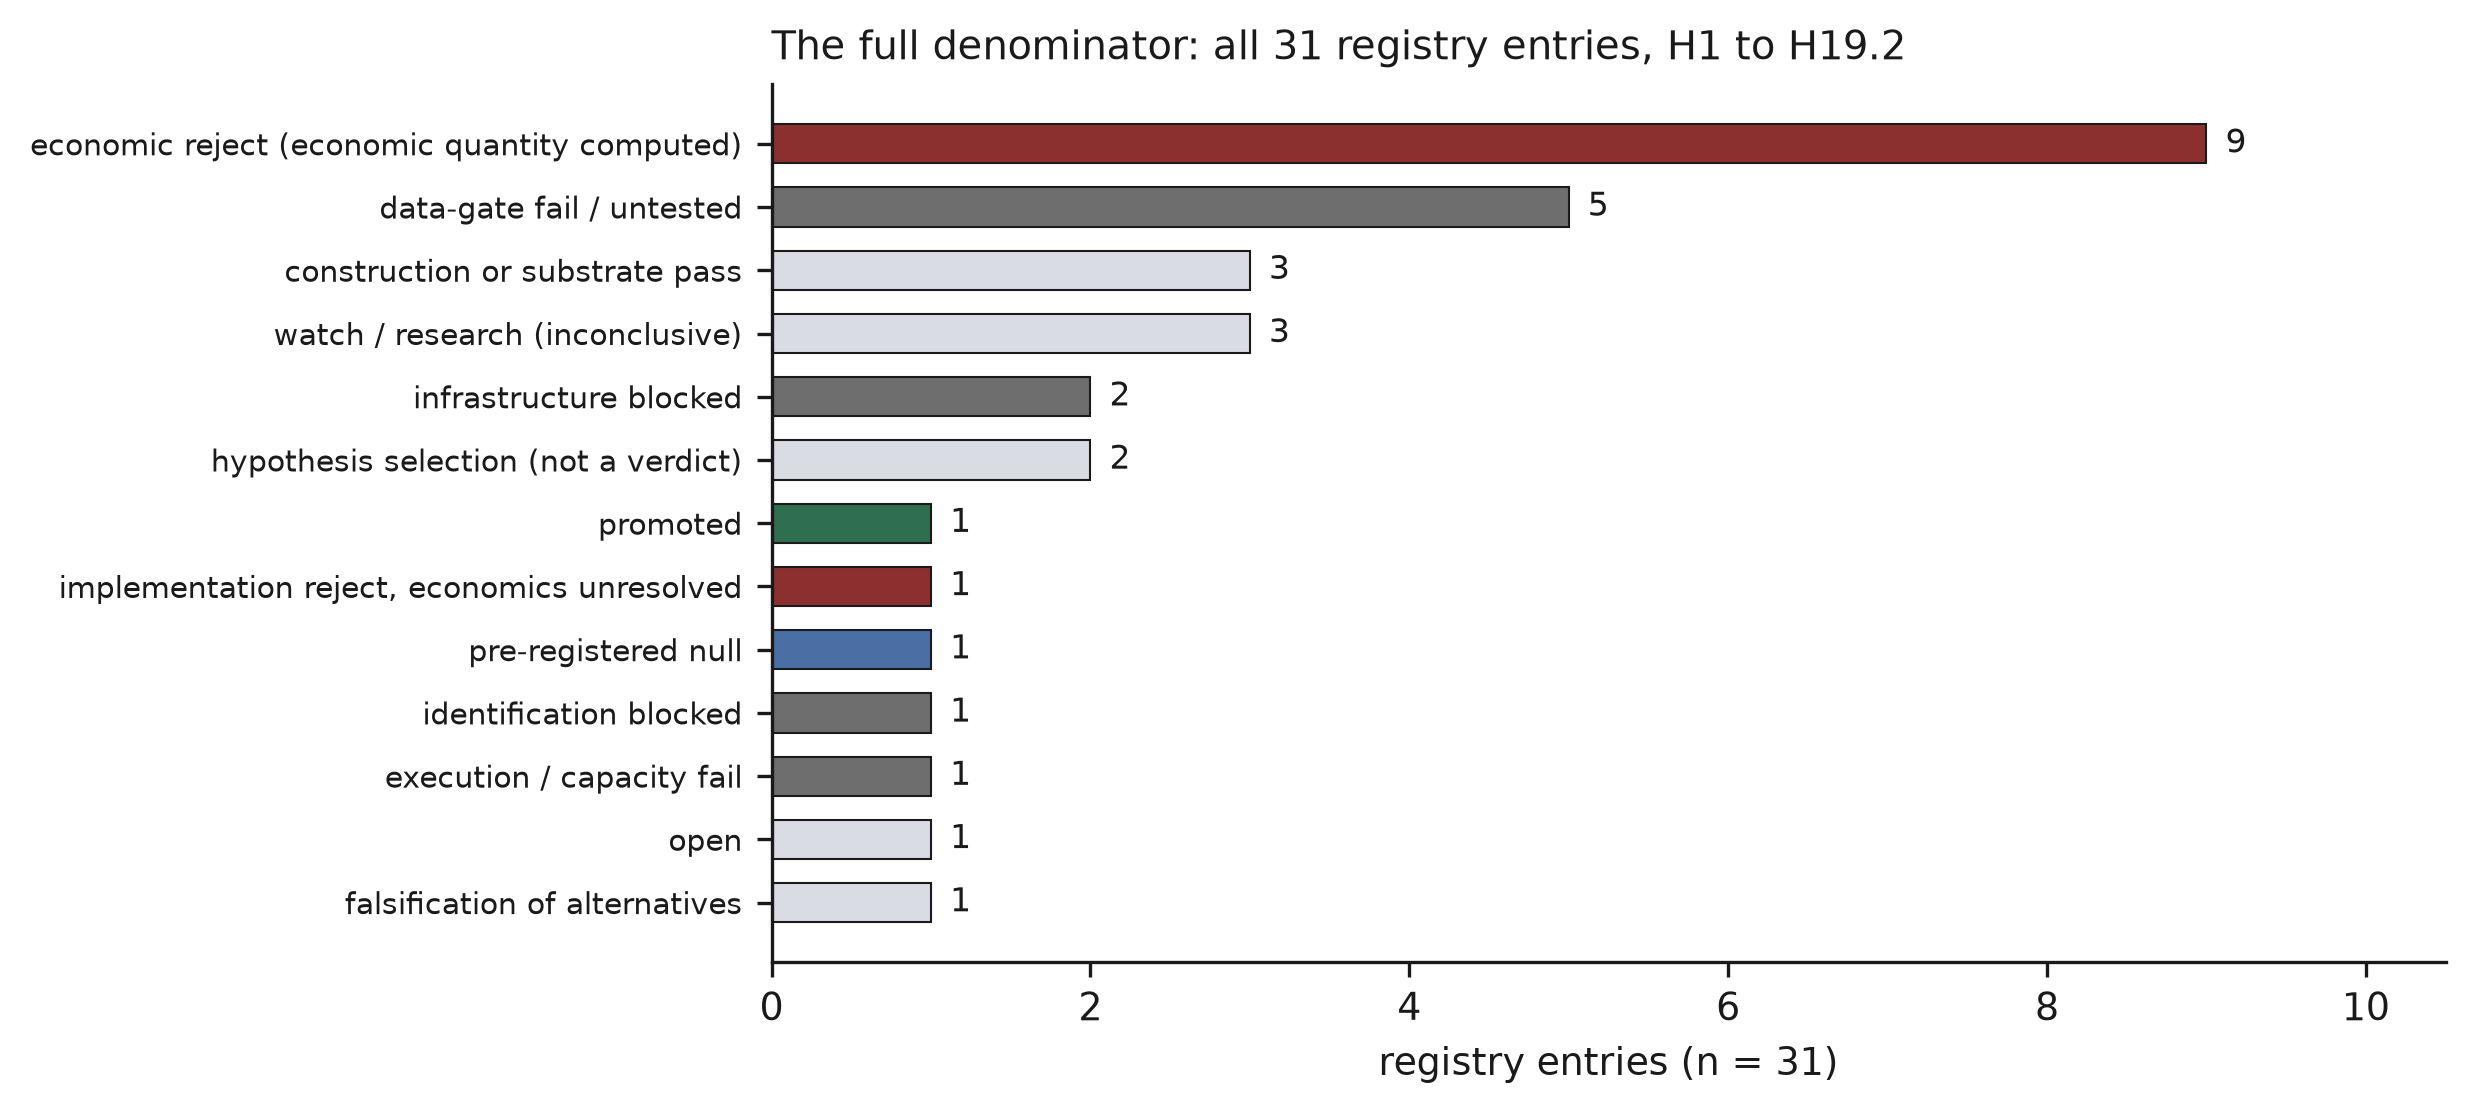
\includegraphics[width=\linewidth]{figures/v2_f1_registry_denominator.png}
\end{center}


\textbf{Figure 1. The full registry denominator.} All n = 31 registry entries, H1 to H19.2, by terminal state, in entries (counts, not percentages). Descriptive. The nine \texttt{economic reject} entries are families in which an economic quantity was computed and the verdict came from it; they are the denominator against which the four detailed case studies should be read (\S{}4.4). \emph{Source: \texttt{docs/alpha\_sprint/HYPOTHESIS\_LEDGER.md}, mapped to the paper taxonomy in \S{}4.3. Data: \texttt{figures/data/v2\_f1\_registry\_denominator.csv}.}


\begin{center}
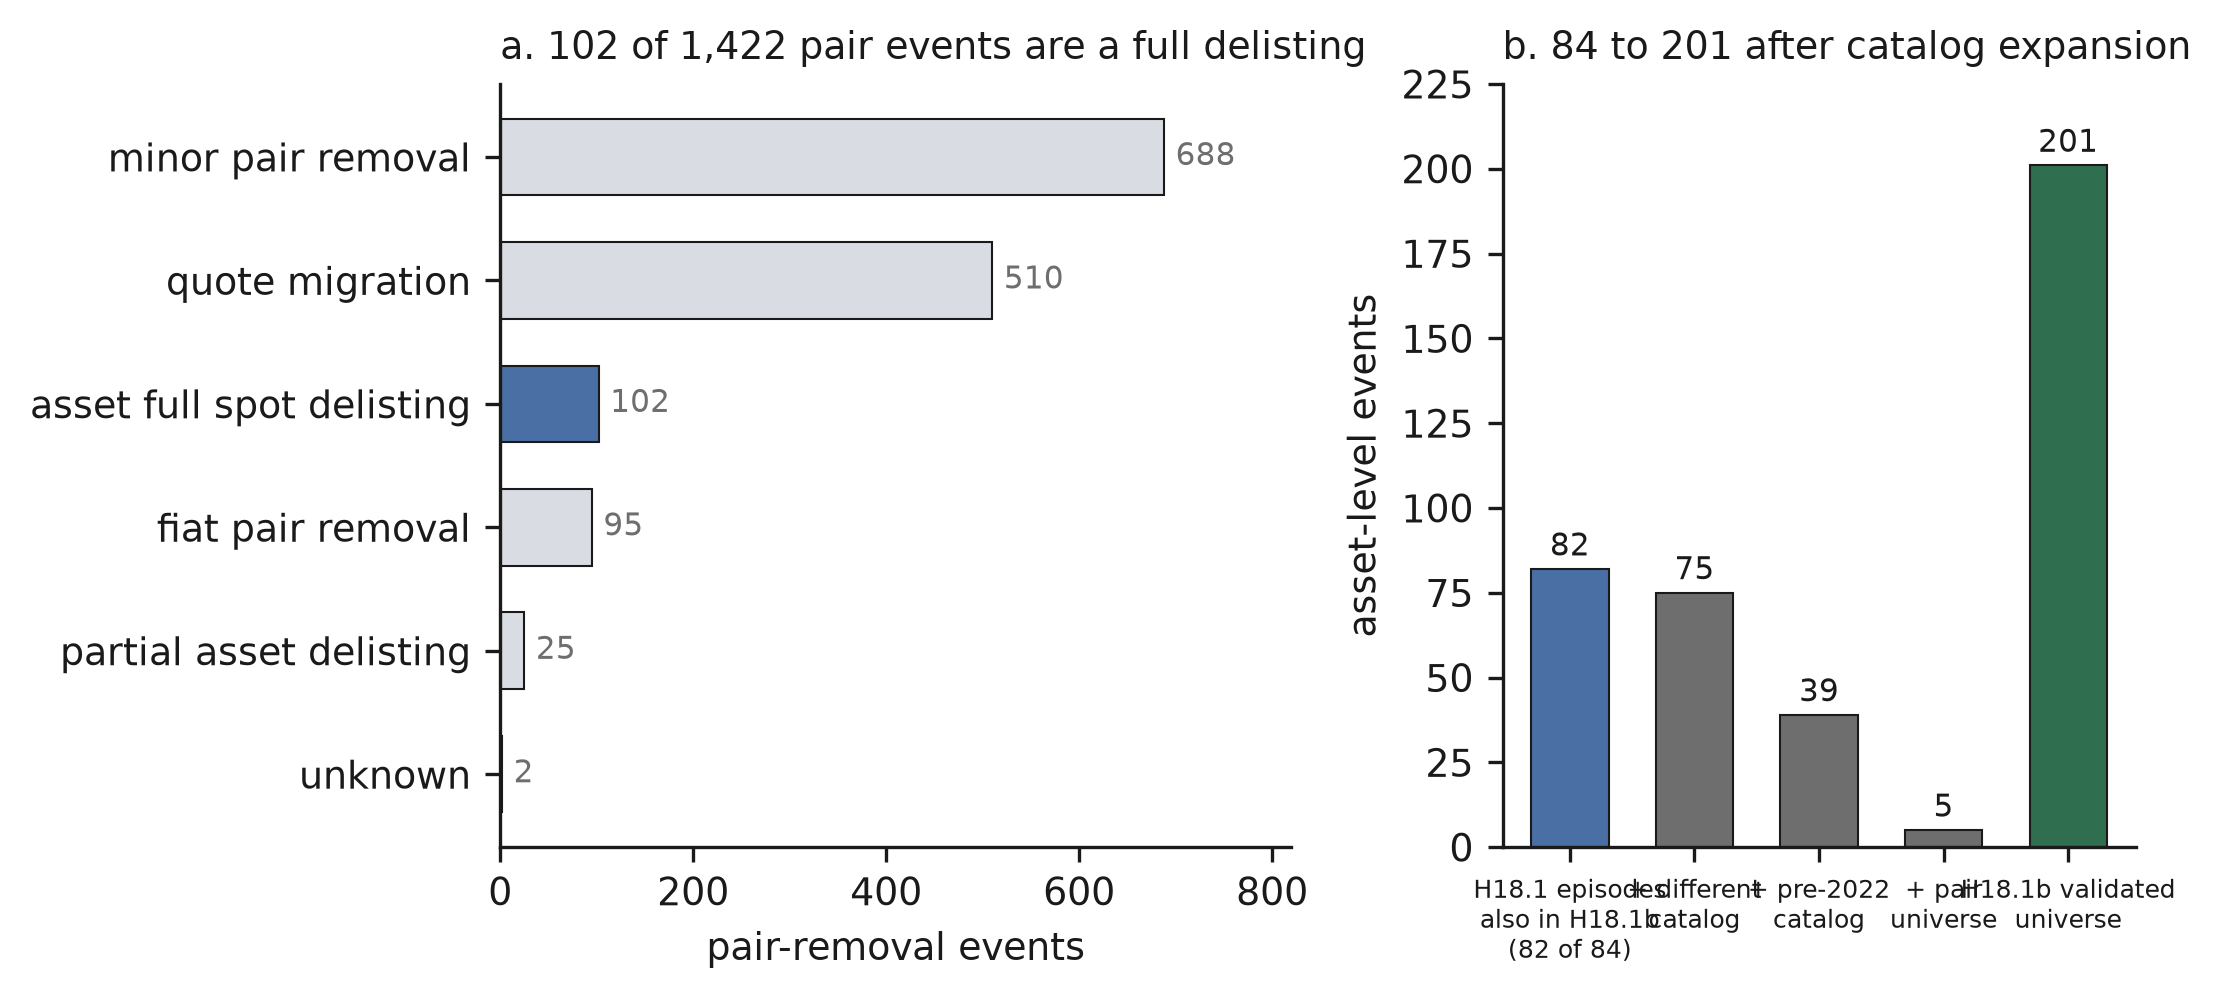
\includegraphics[width=\linewidth]{figures/v2_f3_lifecycle_reconstruction.png}
\end{center}


\textbf{Figure 2. Lifecycle reconstruction.} (a) Classification of n = 1,422 pair-removal events, in events; 102 (7.2\%) are an asset leaving spot entirely. (b) Decomposition of the validated universe, in asset-level events: 82 episodes shared with the earlier construction plus 75 + 39 + 5 recovered events give 201. Descriptive. Recall against candle-measured cessation is 0.9801 (\S{}5.3). \emph{Source: \texttt{H18\_1\_GATE.json}, \texttt{H18\_1B\_GATE.json}. Data: \texttt{figures/data/v2\_f3\_lifecycle\_reconstruction.csv}.}


\begin{center}
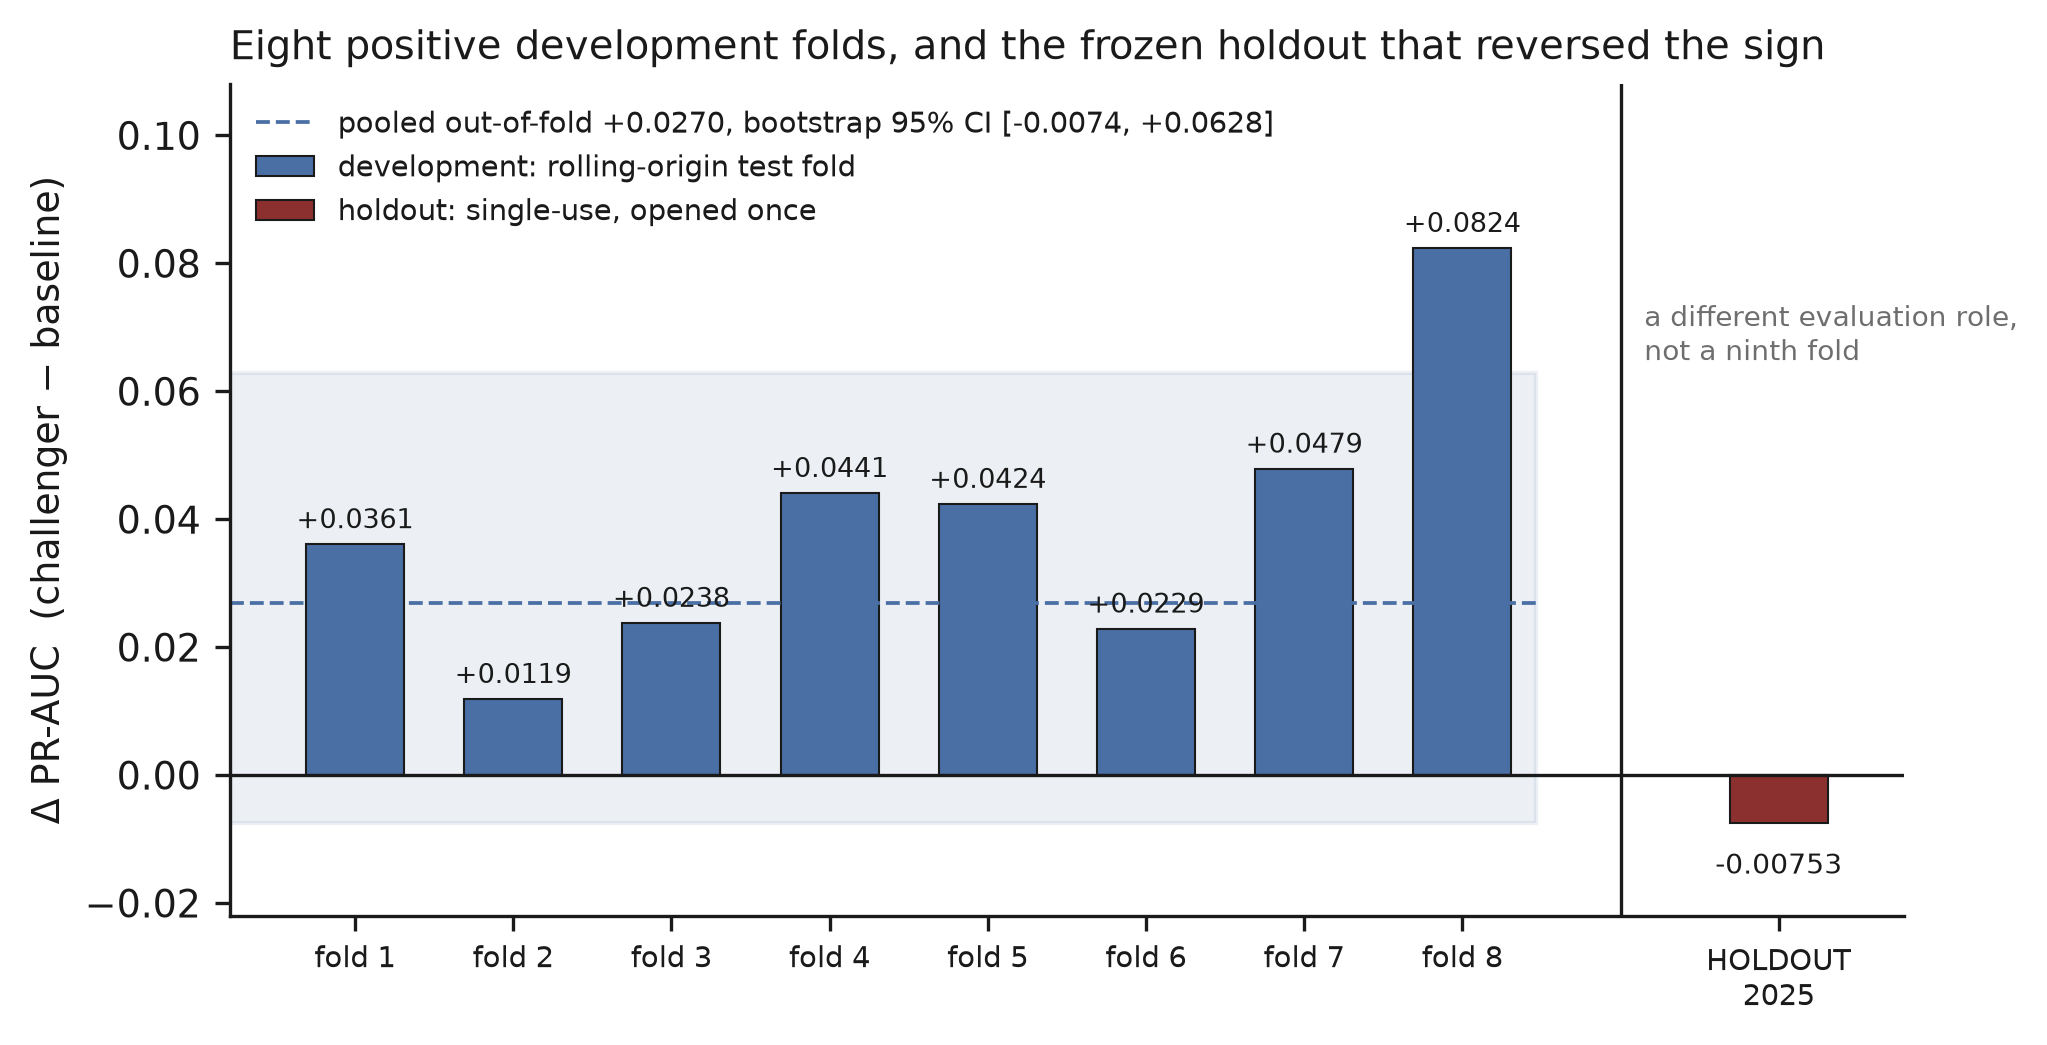
\includegraphics[width=\linewidth]{figures/v2_f4_h18_3_folds_vs_holdout.png}
\end{center}


\textbf{Figure 3. Rolling-origin development folds and the single-use holdout.} $\Delta$PR-AUC (challenger minus baseline), dimensionless. Confirmatory: this is the pre-registered primary metric. Eight development folds (n = 110 unique outcome events, base rate 5.822\%) against the holdout (n = 86 events, base rate 11.792\%), which is drawn apart because it has a different evaluation role and is \textbf{not} a ninth fold. The shaded band is the cluster-bootstrap 95\% interval over asset-eras, [$-$0.0074, +0.0628]; it includes zero, which is why the pre-registered support criterion fails, and it is also consistent with a modest positive effect (\S{}6.3). \emph{Source: \texttt{H18\_3\_DEVELOPMENT\_REPORT.md} \S{}3, \texttt{h18\_3\_development.json}, \texttt{H18\_3\_GATE.json}. Data: \texttt{figures/data/v2\_f4\_h18\_3\_folds\_vs\_holdout.csv}.}


\begin{center}
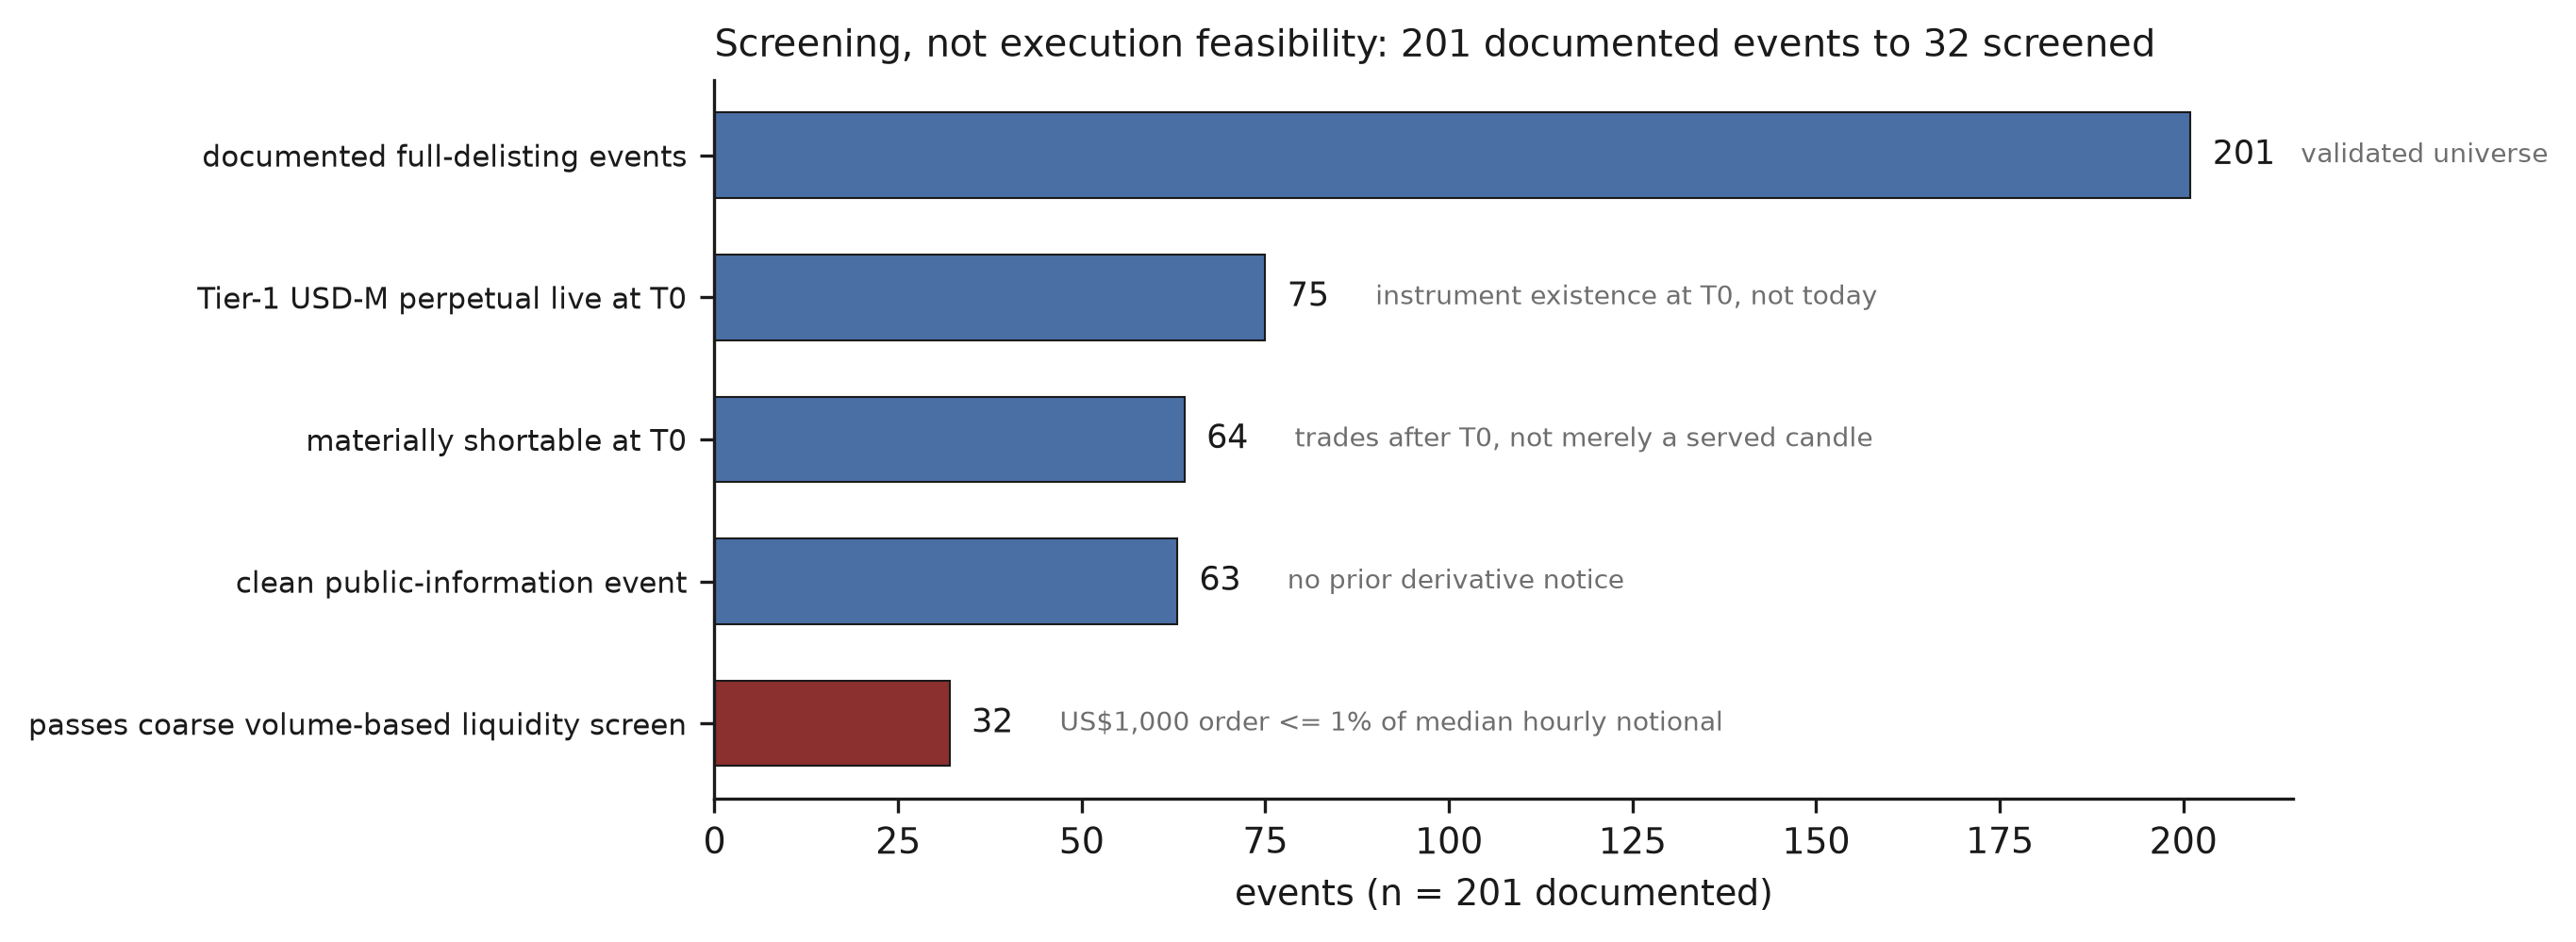
\includegraphics[width=\linewidth]{figures/v2_f5_screening_funnel.png}
\end{center}


\textbf{Figure 4. Screening, not execution feasibility.} Events, from n = 201 documented full-delisting events to 32. Descriptive. The final step is a coarse volume-based liquidity screen (a US\$1,000 order at most 1\% of median hourly notional), \textbf{not} an execution-feasibility test: no order book, spread, impact, fee, funding, latency or fill-probability measurement was available (\S{}7). \emph{Source: \texttt{H19\_0\_GATE.json}. Data: \texttt{figures/data/v2\_f5\_screening\_funnel.csv}.}


\begin{center}
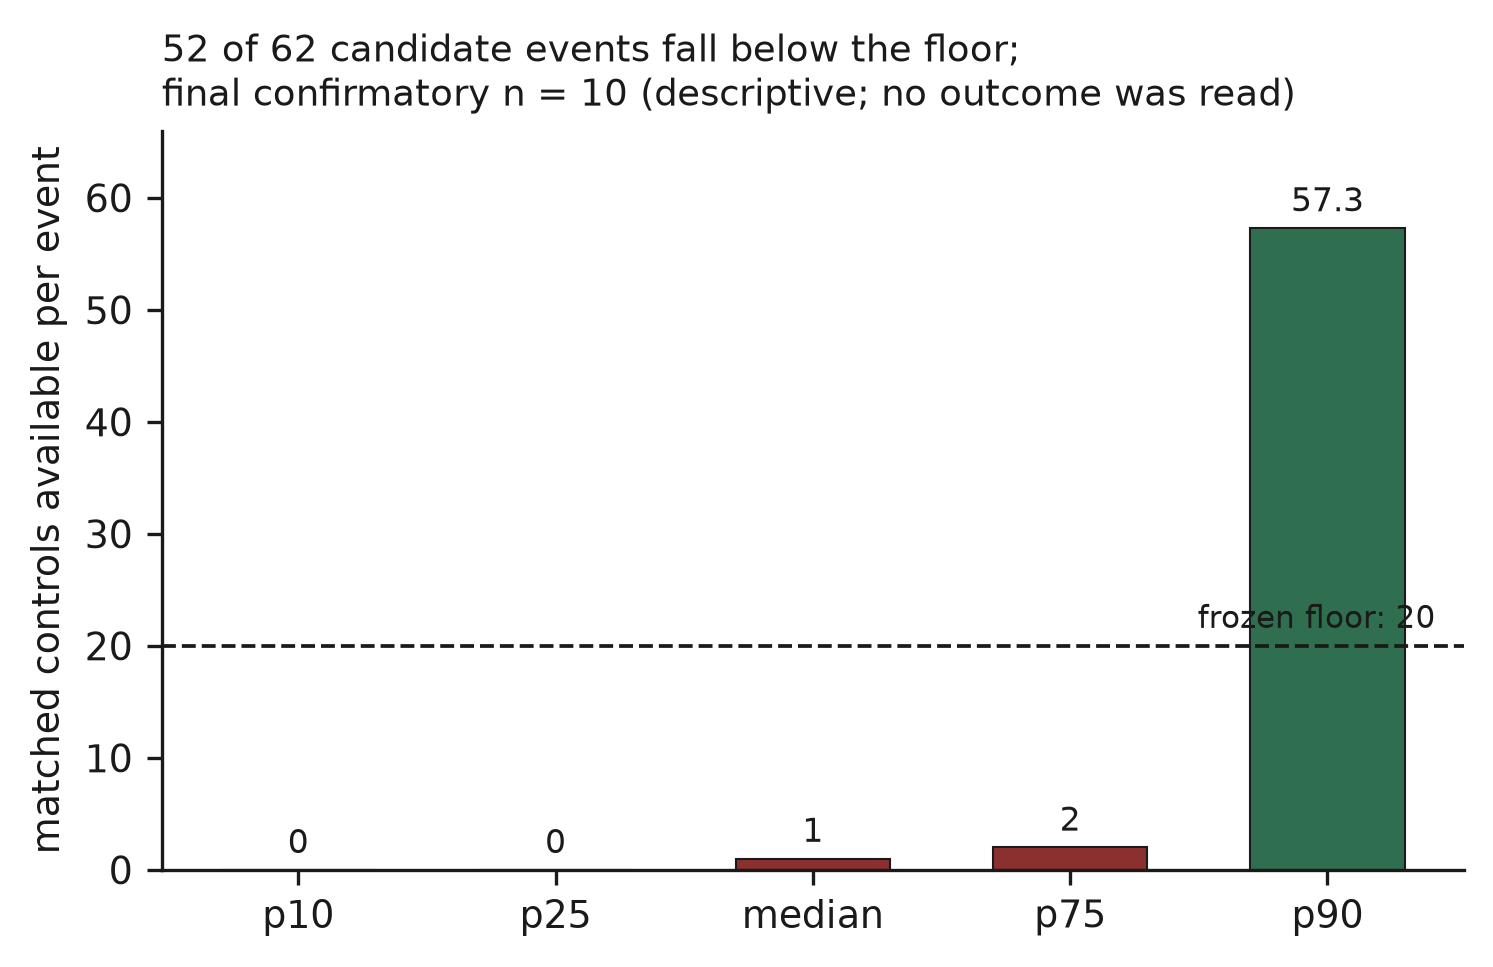
\includegraphics[width=\linewidth]{figures/v2_f6_common_support.png}
\end{center}


\textbf{Figure 5. Realised common support against the frozen floor.} Matched controls available per event, in controls, over the n = 62 candidate events. Descriptive; no outcome column was read. 52 of 62 events fall below the pre-registered floor of 20, leaving a final confirmatory n = 10. The distribution is bimodal: events whose asset was not publicly warned find large pools, and 52 of the 62 event assets were warned (\S{}8.2). \emph{Source: \texttt{data/alpha\_sprint/h19\_2\_prefreeze.json}. Data: \texttt{figures/data/v2\_f6\_common\_support.csv}.}


\subsection*{Appendix figure}


\begin{center}
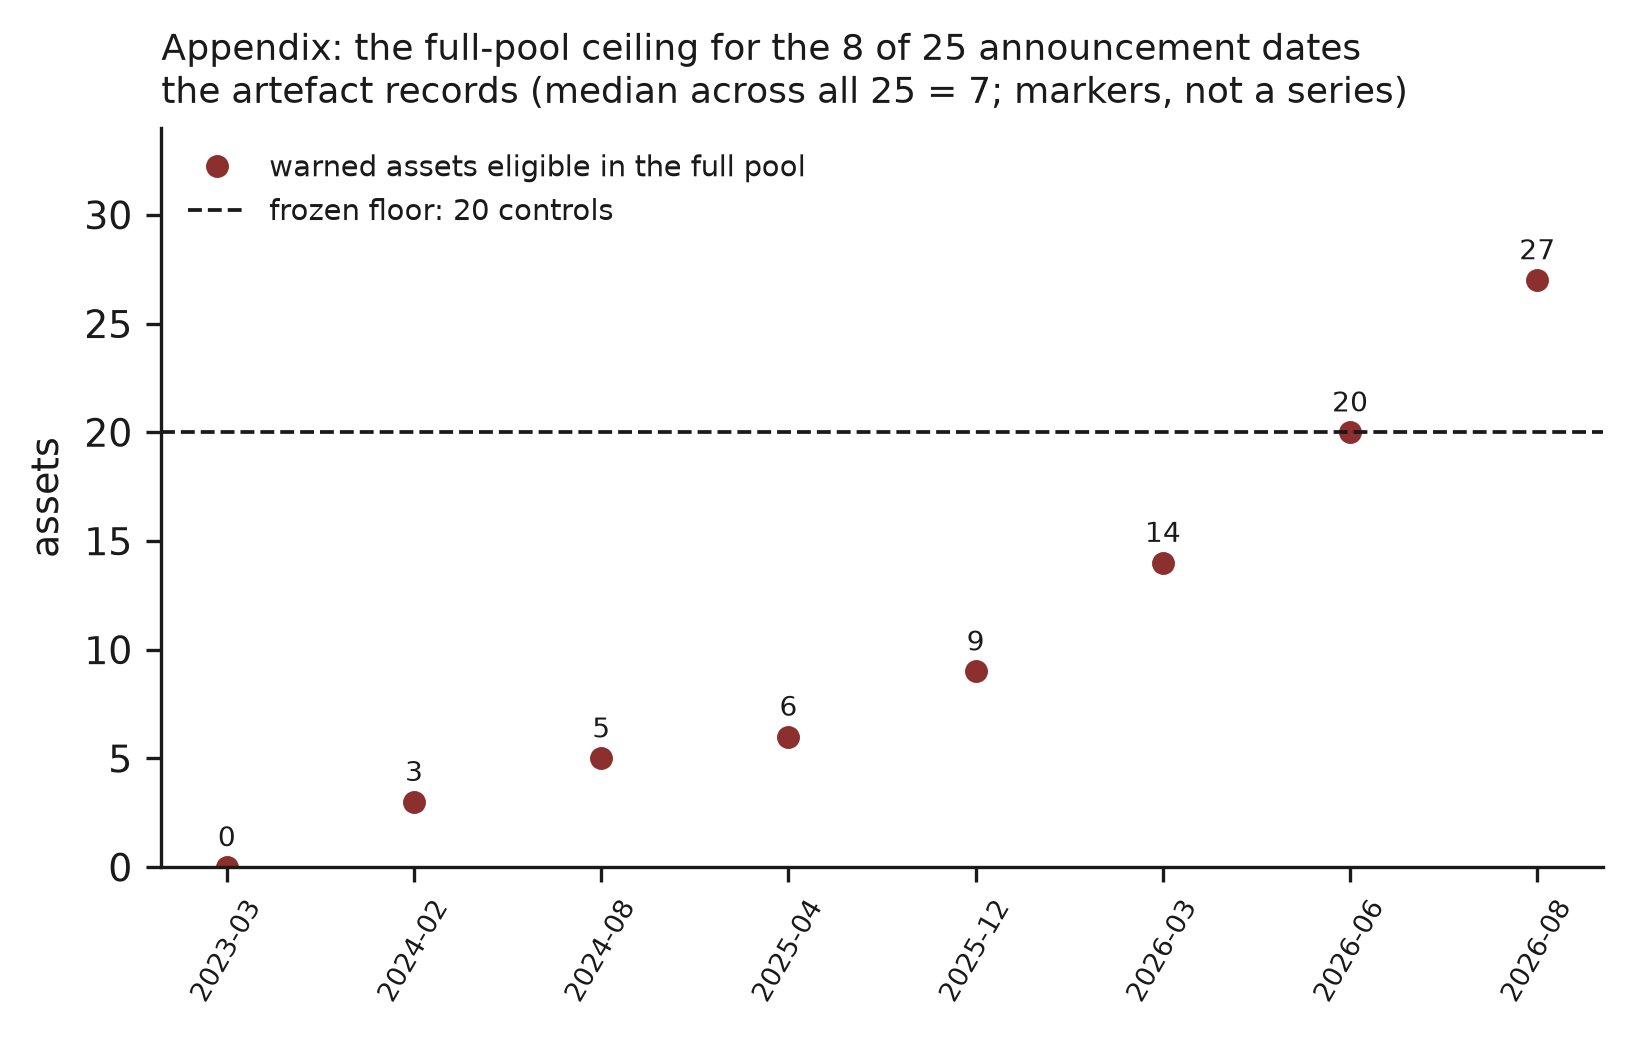
\includegraphics[width=\linewidth]{figures/v2_a1_ceiling.png}
\end{center}


\textbf{Figure A1. The full-pool ceiling.} Warned assets simultaneously eligible as controls, in assets, at each announcement date. Descriptive, computed on the complete eligible pool with no sampling. Markers, not a connected series: the artefact records 8 of the 25 announcement dates, and the remaining 17 were summarised to a median (7) rather than persisted, so the gaps are a limit of the record and are not interpolated. Only 3 of 25 dates reach the floor of 20, before the liquidity band is matched (\S{}8.2). \emph{Source: \texttt{H19\_2\_PREFREEZE\_FEASIBILITY.md} Check 3. Data: \texttt{figures/data/v2\_a1\_ceiling.csv}.}


\section*{Tables}


\begin{center}
\footnotesize
\begin{tabular}{p{0.307\linewidth}p{0.307\linewidth}p{0.307\linewidth}}
\hline
\textbf{\#} & \textbf{table} & \textbf{file} \\
\hline
T1 & experiment registry with gate counts & \texttt{tables/table1\_experiment\_registry.md} \\
T2 & research failure taxonomy & \texttt{tables/table2\_failure\_taxonomy.md} \\
T3 & classes of silent failure & \texttt{tables/table3\_silent\_failure\_classes.md} \\
T4 & H18.3 pre-registered metrics & \texttt{tables/table4\_h18\_3\_preregistered\_metrics.md} \\
T5 & H19 execution and feasibility gate & \texttt{tables/table5\_h19\_execution\_gate.md} \\
\hline
\end{tabular}
\end{center}


The full registry denominator (\S{}4.2), the terminal-state distribution (\S{}4.3) and the threshold classification (\S{}9) are authored in this manuscript rather than generated, because each maps artefact values onto a taxonomy defined here.


\section*{Data and code availability}


Every number in this paper maps to a row of \texttt{CLAIM\_EVIDENCE\_MATRIX\_V2.csv}. Artefacts, commits and hashes are indexed in \texttt{ARTIFACT\_INDEX.md}; environment, seeds and state transitions are in \texttt{REPRODUCIBILITY\_APPENDIX.md}. Tables and figures regenerate from committed artefacts by \texttt{scripts/paper\_build\_tables.py} and \texttt{scripts/paper\_build\_figures.py}; the four audits run by \texttt{scripts/paper\_audit.py}. \textbf{No public repository or DOI exists yet}, which is a limitation for a paper of this kind and a blocking item before any external release.


\section*{Evidence classes}


Four categories, never blended: \textbf{internal empirical evidence} (this program's experiments), \textbf{external literature} (academic work, with access level flagged per entry), \textbf{official venue documentation} (the venue's own published surfaces), and \textbf{paid reference} (cited for context only, never as the evidence that allows a gate to pass; none is used in this paper).


\section*{References}


See \texttt{references\_v2.bib}.



\section*{Appendix A --- Full registry}


See \S{}4.2.


\section*{Appendix B --- Implementation defects, retained for completeness}


Not claimed as contributions. Each produced plausible output and was repaired; none generalises beyond its implementation, and discovering them carries no information about markets.


\begin{center}
\footnotesize
\begin{tabular}{p{0.460\linewidth}p{0.460\linewidth}}
\hline
\textbf{defect} & \textbf{effect} \\
\hline
NaN treated as truthy in an identity guard & 125 valid mappings rejected \\
regular expression matching a product word inside a longer title & one legitimate announcement covering five assets deleted \\
pagination continued from a marker the storage service returns only when a delimiter is set & listing stopped at the 1,000 oldest keys \\
placebo shift not a multiple of the landmark period & zero placebo coverage; corrected to 1,092 days \\
two falsification variants specified with identical feature sets & one redefined to the narrowest count-only variant \\
numerical overflow in a logistic link & caught at runtime; fixed; development re-run; every reported number unchanged to four decimals \\
\hline
\end{tabular}
\end{center}


\end{document}
